%
%  For more information, please see: http://software.sci.utah.edu
% 
%  The MIT License
% 
%  Copyright (c) 2004 Scientific Computing and Imaging Institute,
%  University of Utah.
% 
%  License for the specific language governing rights and limitations under
%  Permission is hereby granted, free of charge, to any person obtaining a
%  copy of this software and associated documentation files (the "Software"),
%  to deal in the Software without restriction, including without limitation
%  the rights to use, copy, modify, merge, publish, distribute, sublicense,
%  and/or sell copies of the Software, and to permit persons to whom the
%  Software is furnished to do so, subject to the following conditions:
% 
%  The above copyright notice and this permission notice shall be included
%  in all copies or substantial portions of the Software.
% 
%  THE SOFTWARE IS PROVIDED "AS IS", WITHOUT WARRANTY OF ANY KIND, EXPRESS
%  OR IMPLIED, INCLUDING BUT NOT LIMITED TO THE WARRANTIES OF MERCHANTABILITY,
%  FITNESS FOR A PARTICULAR PURPOSE AND NONINFRINGEMENT. IN NO EVENT SHALL
%  THE AUTHORS OR COPYRIGHT HOLDERS BE LIABLE FOR ANY CLAIM, DAMAGES OR OTHER
%  LIABILITY, WHETHER IN AN ACTION OF CONTRACT, TORT OR OTHERWISE, ARISING
%  FROM, OUT OF OR IN CONNECTION WITH THE SOFTWARE OR THE USE OR OTHER
%  DEALINGS IN THE SOFTWARE.
%


\documentclass[11pt,titlepage]{book}
\usepackage[]{html}
\usepackage[]{graphicx}
\usepackage[]{alltt}
\usepackage{makeidx}

\usepackage{scirun-doc}
% -*-latex-*-
%
%  The contents of this file are subject to the University of Utah Public
%  License (the "License"); you may not use this file except in compliance
%  with the License.
%
%  Software distributed under the License is distributed on an "AS IS"
%  basis, WITHOUT WARRANTY OF ANY KIND, either express or implied. See the
%  License for the specific language governing rights and limitations under
%  the License.
%
%  The Original Source Code is SCIRun, released March 12, 2001.
%
%  The Original Source Code was developed by the University of Utah.
%  Portions created by UNIVERSITY are Copyright (C) 2001, 1994
%  University of Utah. All Rights Reserved.
%

%
% Recommened markup for latex docs.
%
                                %
% (Mostly) Short cuts  ==============================
\newcommand{\SCI}{{\em SCI}}
\newcommand{\sci}{\SCI}
\newcommand{\scii}{SCI Institute}
\newcommand{\BIOPSE}{{\em BioPSE}}
\newcommand{\biopse}{\BIOPSE}
\newcommand{\SR}{{\em SCIRun}}
\newcommand{\sr}{\SR}
\newcommand{\eg}{{\em e.g.,}}
\newcommand{\ie}{{\em i.e.,}}
\newcommand{\etc}{{\em etc.}}
\newcommand{\etal}{{\em et al.}}
\newcommand{\degrees}{{$^{\circ}$}}
\newcommand{\splitline}{\begin{center}\rule{\columnwidth}{.7mm}\end{center}}
\newcommand{\X}[1]{#1\index{#1}}
\newcommand{\rob}{Rob MacLeod (macleod@cvrti.utah.edu)}
\newcommand{\ted}{Ted Dustman (dustman@cvrti.utah.edu)}
\newcommand{\blythe}{Blythe D Nobleman (blythe@cs.utah.edu)}
\newcommand{\srig}{\sr{} Installation Guide}
\newcommand{\srug}{\sr{} User's Guide}
\newcommand{\srdg}{\sr{} Developer's Guide}

% Literal ~ character
\newcommand{\ltilde}{\textasciitilde}

% Encloses its argument between angle brackets.
\newcommand{\ab}[1]{\latexhtml{\textless{}#1\textgreater}{<#1>}}

% Inserts a left angle bracket.
\newcommand{\la}{\latexhtml{\textless}{<}}

% Inserts a right angle bracket.
\newcommand{\ra}{\latexhtml{\textgreater}{>}}

% Mark up commands =================================

% Url
%\newcommand{\url}[1]{#1}

% ip address
\newcommand{\ipaddr}[1]{#1}
\newcommand{\localhost}{\ipaddr{127.0.0.1}}

% Acronym
\newcommand{\acronym}[1]{#1}

% Predefined acronyms
\newcommand{\gui}{\acronym{GUI}}
\newcommand{\tcl}{\acronym{TCL}}
\newcommand{\xml}{\acronym{XML}}
\newcommand{\pse}{\acronym{PSE}}

% Markup the first time use of term that may be unfamiliar to the
% reader. 
\newcommand{\dfn}[1]{\emph{#1}}

% In the next command #1 is the term and #2 is the shortcut or acronym that
% will be used in the rest of the document. 
\newcommand{\dfna}[2]{\emph{#1} (#2)}

% Directory name markup.
\newcommand{\directory}[1]{\texttt{#1}}

% Markup a file name.
\newcommand{\filename}[1]{\texttt{#1}}

% Markup text which is the name of a command.
\newcommand{\command}[1]{\texttt{#1}} 

% Command option.
\newcommand{\option}[1]{\texttt{#1}}

% Markup text typed at the keyboard.
\newcommand{\keyboard}[1]{\texttt{#1}} 

% Parameterized text - marks up text that is to be
% substituted for by the reader.
\newcommand{\ptext}[1]{\textit{#1}}

% Markup text the user might see on his screen.
\newcommand{\screen}[1]{\texttt{#1}}

% Markup the name of a GUI menu.
\newcommand{\guimenu}[1]{\textbf{#1}}

% Markup the name of a GUI menu.
\newcommand{\menu}[1]{\guimenu{#1}}

% Markup a gui menu item name.
\newcommand{\guimenuitem}[1]{\textbf{#1}}

% Markup a menu item name.
\newcommand{\menuitem}[1]{\guimenuitem{#1}}

% Markup name of a ui button.
\newcommand{\guibutton}[1]{\textbf{#1}}

% Markup name of a ui button.
\newcommand{\button}[1]{\guibutton{#1}}

% Markup name of a gui text item.
\newcommand{\guitext}[1]{\textit{#1}}

% Markup name of a gui label.
\newcommand{\guilabel}[1]{\textbf{#1}}

% GUI variable
\newcommand{\guivar}[1]{\texttt{#1}}

% Scirun port
\newcommand{\srport}[1]{\texttt{#1}}

% Sockets port
\newcommand{\port}[1]{\texttt{#1}}

% Socket
\newcommand{\socket}[2]{\texttt{#1:#2}}

% Variable
\newcommand{\variable}[1]{\texttt{#1}}

% Data type
\newcommand{\datatype}[1]{\texttt{#1}}

% Markup an inline code fragment.
\newcommand{\icode}[1]{\texttt{#1}}

% Markup a module name.
\newcommand{\module}[1]{\texttt{#1}}

% Markup a sr package name.
\newcommand{\package}[1]{\texttt{#1}}

% Markup a sr category name.
\newcommand{\category}[1]{\texttt{#1}}

% Call attention to some useful bit of information.
\newcommand{\note}[1]{\emph{Note: #1}} 

% Call attention to a warning.
\newcommand{\warning}[1]{\emph{Warning: #1}} 

% Call attention to a tip.
\newcommand{\tip}[1]{\emph{Tip: #1}} 

% Env variable markup.
\newcommand{\envvar}[1]{\texttt{#1}}

% Markup for the title of a book or article or whatever.
\newcommand{\etitle}[1]{\texttt{#1}}

% Markup name of a latex section.  First arg is section name.  Second arg
% is section's label.  When processed with latex, the section
% name is emphasized.  When processed with latex2html section name is made
% into a link to section.
\newcommand{\secname}[2]{\latexhtml{\emph{#1}}{\htmlref{#1}{#2}}}

% Section ref command.  Use of this command
% in place of \ref to reference sections (subsections etc.) will
% create a more web friendly version of your document.
% The command's first argument is the link text (used only on the html
% page) and the second argument is the section's label
\newcommand{\secref}[2]{\hyperref[ref]{\emph{#1}}{Section~}{}{#2}}

% A latex command
\newcommand{\latexcommand}[1]{\texttt{\textbackslash#1}}

% A latex package
\newcommand{\latexpackage}[1]{\textit{#1}}

% Use these in place of missing content.
\newcommand{\missing}[1]{\emph{#1 - Coming Soon.}}

% Use this to make note of incomplete content.
\newcommand{\incomplete}{\emph{More Comming Soon.}}

% Mark up a mail address
\newcommand{\mailto}[1]{\texttt{#1}}

% Sci Urls ========================================= 

% www style urls.
\newcommand{\scisoftware}{http://software.sci.utah.edu}
\newcommand{\scisoftwareurl}{\htmlurl{\scisoftware}}
\newcommand{\sciurl}{\htmlurl{http://www.sci.utah.edu}}
\newcommand{\scidocurl}{\htmlurl{\scisoftware{}/doc}}
\newcommand{\scidocurlplus}[1]{\htmlurl{\scisoftware{}/doc/#1}}
\newcommand{\bugsurl}{\htmlurl{\scisoftware{}/bugzilla}}
\newcommand{\scisoftwarearchiveurl}{\htmlurl{\scisoftware{}/archive\_entry.html}}

% -*-latex-*-
% Document name: /u/srug/srugmacros.tex
% Creator: Rob MacLeod [macleod@cvrti.utah.edu]
% Last update: Tue Mar  6 14:33:05 2001 by Rob MacLeod
%    - created from things in the style file that latex2html could not
%      find.
% Creation Date: Wed Feb 21 23:50:38 2001
%%%%%%%%%%%%%%%%%%%%%%%%%%%%%%%%%%%%%%%%%%%%%%%%%%%%%%%%%%%%%%%%%%%%%%
% Markup and other useful text substitution commands.

% (Mostly) Short cuts  ==============================
\newcommand{\SCI}{\emph{SCI}}
\newcommand{\sci}{\SCI}
\newcommand{\scii}{SCI Institute}
\newcommand{\PSE}{\emph{BioPSE}}
\newcommand{\pse}{\PSE}
\newcommand{\SR}{\emph{SCIRun}}
\newcommand{\sr}{\SR}
\newcommand{\eg}{{\em e.g.,}}
\newcommand{\ie}{{\em i.e.,}}
\newcommand{\etc}{{\em etc.,}}
\newcommand{\etal}{{\em et al.}}
\newcommand{\degrees}{{$^{\circ}$}}
\newcommand{\splitline}{\begin{center}\rule{\columnwidth}{.7mm}\end{center}}
\newcommand{\X}[1]{#1\index{#1}}
\newcommand{\version}{1.1}
\newcommand{\rob}{Rob MacLeod (macleod@cvrti.utah.edu)}
\newcommand{\ted}{Ted Dustman (dustman@cvrti.utah.edu)}
\newcommand{\srug}{\sr{} User's Guide}
\newcommand{\srig}{\sr{} Installation Guide}
\newcommand{\viewer}{\emph{Viewer}}

% Literal ~ character
\newcommand{\ltilde}{\symbol{'176}}

% Encloses its argument between angle brackets.
\newcommand{\ab}[1]{\latexhtml{$<$#1$>$}{<#1>}}

% Inserts a left angle bracket.
\newcommand{\la}{\latexhtml{$<$}{<}}

% Inserts a right angle bracket.
\newcommand{\ra}{\latexhtml{$>$}{>}}

% Urls =============================================

% www style urls.
\newcommand{\scisoftwareurl}{http://software.sci.utah.edu}
\newcommand{\sciurl}{http://www.sci.utah.edu}
\newcommand{\scidocurl}{\scisoftwareurl/software}
\newcommand{\bugsurl}{\scisoftwareurl/research/software/bugzilla}

% Urls relative to userguide directory in the distribution.
\newcommand{\installguideurl}{../../InstallGuide/installguide.xml?cont=0\&amp;dir=2}
\newcommand{\modulemakerguideurl}{../../DeveloperGuide/create_module.html}

% Mark up commands =================================

% Acronym
\newcommand{\acronym}[1]{#1}

% Predefined acronyms
\newcommand{\gui}{\acronym{GUI}}
\newcommand{\tcl}{\acronym{TCL}}

% Markup the first time use of term that may be unfamiliar to the
% reader. 
\newcommand{\dfn}[1]{\emph{#1}}
% In the next command #1 is the term and #2 is the shortcut or acronym that
% will be used in the rest of the document. 
\newcommand{\dfna}[2]{\emph{#1} (#2)}

% Directory name markup.
\newcommand{\directory}[1]{\texttt{#1}}

% Markup a file name.
\newcommand{\filename}[1]{\texttt{#1}}

% Markup text which is the name of a command.
\newcommand{\command}[1]{\texttt{#1}} 

% Markup text typed at the keyboard.
\newcommand{\keyboard}[1]{\texttt{#1}} 

\newcommand{\ptext}[1]{\textit{\ab{#1}}}

% Markup text the user might see on his screen.
\newcommand{\screen}[1]{\texttt{#1}}

% Markup the name of a menu.
\newcommand{\menu}[1]{\textbf{#1}}

% Markup a menu item name.
\newcommand{\menuitem}[1]{\textbf{#1}}

% Markup name of a ui button.
\newcommand{\button}[1]{\textbf{#1}}

% Markup an inline code fragment.
\newcommand{\icode}[1]{\texttt{#1}}

% Markup a module name.
\newcommand{\module}[1]{\texttt{#1}}

% Markup a sr package name.
\newcommand{\package}[1]{\texttt{#1}}

% Markup a sr category name.
\newcommand{\category}[1]{\texttt{#1}}

% Call attention to some useful bit of information.
\newcommand{\note}[1]{\emph{Note: #1}} 

% Call attention to a warning.
\newcommand{\warning}[1]{\emph{Warning: #1}} 

% Call attention to a tip.
\newcommand{\tip}[1]{\emph{Tip: #1}} 

% Env variable markup.
\newcommand{\envvar}[1]{\texttt{#1}}

% Markup for the title of a book or article or whatever.
\newcommand{\etitle}[1]{\texttt{#1}}

% Section command.  This command should be
% used in place of \ref to reference sections (subsections etc.).
% The command's first argument is the link text (used only on the html
% page) and the second argument is the section's label
\newcommand{\secref}[2]{\hyperref[ref]{\emph{#1}}{Section~}{}{#2}}

% Use these in place of missing content.
\newcommand{\missing}[1]{\emph{#1 - Coming Soon.}}

% Use this to make note of incomplete content.
\newcommand{\incomplete}{\emph{More Comming Soon.}}

% Mark up a mail address
\newcommand{\mailto}[1]{\texttt{#1}}

%%% Local Variables: 
%%% mode: latex
%%% TeX-master: "usersguide"
%%% End: 
 

\makeindex
\newcommand{\clearemptydoublepage}{\newpage{\pagestyle{empty}\cleardoubleapage}}
\begin{document}

% -*-latex-*-
% Document name: title.tex
% Creator: Rob MacLeod [macleod@cvrti.utah.edu]
% Last update: Thu Feb 22 00:04:50 2001 by Rob MacLeod
%    - created
%%%%%%%%%%%%%%%%%%%%%%%%%%%%%%%%%%%%%%%%%%%%%%%%%%%%%%%%%%%%%%%%%%%%%%
  \mbox{}
  \vspace{2in}
\begin{center}
   {\huge\bf \PSE{} User's Guide}\\
     \vspace{.5in}
     {\Large Version \version{} \\
     \medskip
     Last update: \today \\}
     \bigskip
     {\Large Authors: \htmladdnormallink{\rob{}}
     {mailto:macleod@cvrti.utah.edu}, \\
     \htmladdnormallink{\ted{}}
     {mailto:dustman@cvrti.utah.edu}, \\
     and the SCI Gang\\}
  \bigskip

     {\Large 
     Scientific and Computing Institute (SCI)\\
     \htmladdnormallink{www.sci.utah.edu}{http://www.sci.utah.edu/}\\
     \medskip
     Nora Eccles Harrison \\
     Cardiovascular Research and Training Institute (CVRTI)\\
  %   \smallskip
     \htmladdnormallink{www.cvrti.utah.edu}{http://www.cvrti.utah.edu/}\\
     \medskip

     \bigskip
     Support for this project came from:\\
     \medskip
     The NIH National Center for Research Resources  
     \htmladdnormallink{(NCRR)}{http://www.ncrr.nih.gov}}

\end{center}

\pagenumbering{roman}
\tableofcontents
\clearpage
\pagenumbering{arabic}
%
%  For more information, please see: http://software.sci.utah.edu
% 
%  The MIT License
% 
%  Copyright (c) 2004 Scientific Computing and Imaging Institute,
%  University of Utah.
% 
%  License for the specific language governing rights and limitations under
%  Permission is hereby granted, free of charge, to any person obtaining a
%  copy of this software and associated documentation files (the "Software"),
%  to deal in the Software without restriction, including without limitation
%  the rights to use, copy, modify, merge, publish, distribute, sublicense,
%  and/or sell copies of the Software, and to permit persons to whom the
%  Software is furnished to do so, subject to the following conditions:
% 
%  The above copyright notice and this permission notice shall be included
%  in all copies or substantial portions of the Software.
% 
%  THE SOFTWARE IS PROVIDED "AS IS", WITHOUT WARRANTY OF ANY KIND, EXPRESS
%  OR IMPLIED, INCLUDING BUT NOT LIMITED TO THE WARRANTIES OF MERCHANTABILITY,
%  FITNESS FOR A PARTICULAR PURPOSE AND NONINFRINGEMENT. IN NO EVENT SHALL
%  THE AUTHORS OR COPYRIGHT HOLDERS BE LIABLE FOR ANY CLAIM, DAMAGES OR OTHER
%  LIABILITY, WHETHER IN AN ACTION OF CONTRACT, TORT OR OTHERWISE, ARISING
%  FROM, OUT OF OR IN CONNECTION WITH THE SOFTWARE OR THE USE OR OTHER
%  DEALINGS IN THE SOFTWARE.
%


% intro.tex
%

\chapter{Introduction}
\label{ch:intro}

This is the \etitle{\srug}.  It describes the purpose and use of the
\sr{} problem solving environment (\pse).  This guide is for users who
are building and executing \dfn{networks} within the \sr{}
environment.

Users installing \sr{} should read the
\htmladdnormallinkfoot{\srig}{\latexhtml{\scisoftware/doc}{../../..}/Installation/Guide/index.html}.

Users of the BioTensor PowerApp should see the
\htmladdnormallinkfoot{BioTensor
  tutorial}{\latexhtml{\scisoftware/doc/User/Tutorials/BioTensor/BioTensor.html}{../../Tutorials/BioTensor/BioTensor.html}}.

Users of the BioFEM PowerApp should see the
\htmladdnormallinkfoot{BioFEM
  tutorial}{\latexhtml{\scisoftware/doc/User/Tutorials/BioFEM/BioFEM.html}{../../Tutorials/BioFEM/BioFEM.html}}.

Users of the BioImage PowerApp should see the
\htmladdnormallinkfoot{BioImage
  tutorial}{\latexhtml{\scisoftware/doc/User/Tutorials/BioImage/bioimage.html}{../../Tutorials/BioImage/bioimage.html}}.

%\section{Conventions}
%\label{sec:conventions}

%\missing{Discussion of typographic conventions}

\section{Road Map}
\label{sec:roadmap}

This document is organized into the following sections:

\begin{description}
  \descitem{\chref{Introduction}{ch:intro}} This introduction.
  
  \descitem{\chref{Concepts}{ch:concepts}} Introduces the concept of
  an integrated problem solving environment and describes how \SR{}
  embodies these ideas.
  
  \descitem{\chref{Packages}{ch:packages}} Gives an overview
  of the \sr{} and \biopse{} packages.
  
  \descitem{\chref{Starting \sr}{ch:startingup}} Outlines procedure
  for starting \sr{} and related information.

  \descitem{\chref{Working with Networks}{ch:workwithnets}}
  Discusses building, editing, and executing
  networks.

  \descitem{\chref{Visualization}{ch:viewer}}
  Describes the purpose and use of the \viewer{} (visualization) module.

  \descitem{\chref{Importing data into \sr{}}{ch:import_export}}
  Describes ways to import/export ``foreign'' data into/out of \SR{}.

  \descitem{\chref{Wrapping  ITK Filters in \sr{}
      Modules}{ch:itk_mods}}
  Describes the mechanism for wrapping ITK filters in \sr{} modules.
\end{description}

\section{Help}
\label{sec:help}

Help is available from the following sources.

\subsection{Documentation Distribution}

\sr{} documentation is distributed separately from its source code.
\sr{}'s documentation distribution can be downloaded from
\htmladdnormallinkfoot{\sr{}'s software download
  page}{\scisoftwarearchiveurl}.  See the 
\htmladdnormallinkfoot{\srig}{\latexhtml{\scisoftware/doc}{../../..}/Installation/Guide/index.html}
for instructions on downloading and installing the documentation
distribution.

After installing the documentation, visit the
\filename{index.html} file located in the distribution's top level
\directory{doc} directory (\ie{} \ab{top of documentation
  distribution}/doc/index.html).

\subsection{The Web}

This and other documents related to \sr{} can be found 
\htmladdnormallinkfoot{online}{\scidocurl{}}.

Visit the \htmladdnormallinkfoot{\sci}{\sciurl} web site for more
information related to \sr{} and the \scii{}.

\subsection{Mailing Lists}
\index{mailing lists}

The \sr{} \emph{users} mail list is a forum for discussing \sr{}
related issues.  Users are given the opportunity to subscribe to this
list when downloading \sr{} for the first time from the software
download page.  Users may also subscribe by sending mail to:

\mailto{Majordomo@sci.utah.edu}

with the following command in the body of the message:

\keyboard{subscribe scirun-users}

After subscribing,  questions can be sent to
\mailto{scirun-users@sci.utah.edu}.

The \sr{} \emph{developers} list is a forum for network and module
developers.  To subscribe send mail to:

\mailto{Majordomo@sci.utah.edu}

with the following command in the body of the message:

\keyboard{subscribe scirun-develop}

After subscribing, questions can be sent to
\mailto{scirun-develop@sci.utah.edu}.

\section{Reporting Bugs}
\label{sec:bugs}

Please report bugs!  To report a bug visit \sr{}'s
\htmladdnormallinkfoot{bug database}{\bugsurl} web page.

Reporting bugs to the bug database, rather than the mailing list,  ensures
bugs are fixed in a timely manner.

% -*-latex-*-
%
%  The contents of this file are subject to the University of Utah Public
%  License (the "License"); you may not use this file except in compliance
%  with the License.
%
%  Software distributed under the License is distributed on an "AS IS"
%  basis, WITHOUT WARRANTY OF ANY KIND, either express or implied. See the
%  License for the specific language governing rights and limitations under
%  the License.
%
%  The Original Source Code is SCIRun, released March 12, 2001.
%
%  The Original Source Code was developed by the University of Utah.
%  Portions created by UNIVERSITY are Copyright (C) 2001, 1994
%  University of Utah. All Rights Reserved.
%

%%%%%%%%%%  Figures used in this file %%%%%%%%%%%%%%%%%%%%%%%%%%%%%%%%
%begin{latexonly}
  \newcommand{\basicmodule}%
  {\centerline{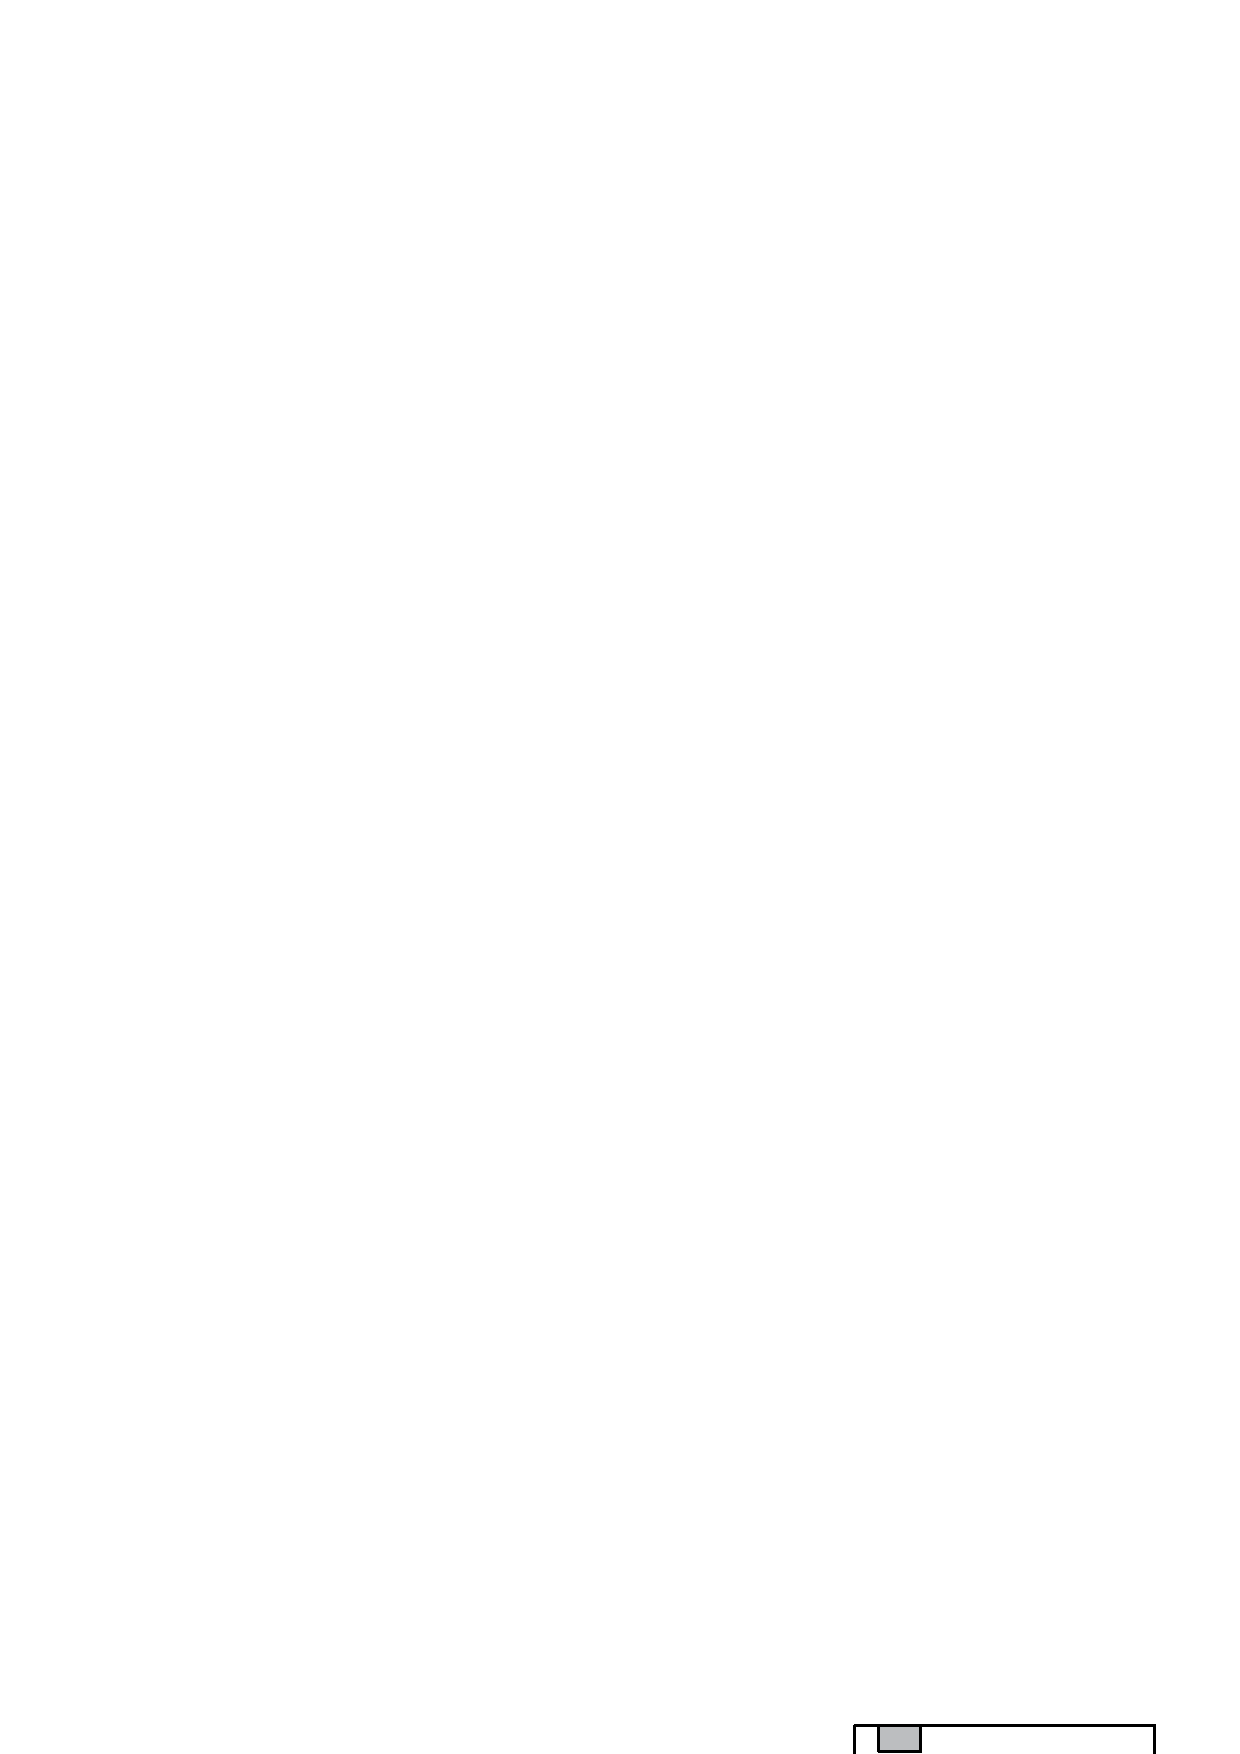
\epsfig{file=Figures/biopse-modmap.eps.gz,width=\columnwidth,
  bbllx=7, bblly=-193, bburx=774, bbury=14}}}
%end{latexonly}
\begin{htmlonly}
  \newcommand{\basicmodule}{%
  \htmladdimg[align=top,width=766,alt="module"]
  {../Figures/biopse-modmap.gif}}
\end{htmlonly}
%%%%%%%%%%%%%%%%%%%%%%%%%%%%%%%%%%%%%%%%%%%%%%%%%%%%%%%%%%%%%%%%%%%%%%
\section{Concepts}
\label{sec:concepts} 
\index{concepts}

Read this section to learn about the design philosphy and goals of
integrated problem solving environments \index{problem solving environment}
generally and how \PSE{} embodies
some of these ideas.  

\subsection{Traditional problem solving methods}

The traditional method for solving bioelectric field problems uses
multiple, non-integrated computer programs.  For example, a scientist using
a computer simulation to examine the effect of electrode patch placement on
transcardiac current density in the design of a cardiac implantable
defibrillator\cite{CRJ:Sch95b} would require geometric modeling, numerical
simulation, and scientific visualization tools to complete the task.  The
user might need one program to define the thoracic surfaces from medical
images and another to create a discrete mesh of the volume contained within
the surfaces\cite{CRJ:Sch93b}.  Another application like Matlab computes a
finite element simulation of the electric current distribution from the
defibrillation electrodes through the thoracic volume\cite{RSM:And93}.
Another approach might be to write a Fortran program using a public domain
numerical library such as LAPACK\@ \index{LAPACK}.  To see the output would
require a scientific visualization package (such as those described
in\cite{RSM:All91}).  Between each of these steps, it would be necessary to
save the output of one program in a format that the next in the sequence
could read---this might necessitate separate file format conversion
utilities.  To find the optimal location, shape, and size parameters for
the defibrillating electrode, the scientist would have to go back to the
geometric modeling package, change the necessary parameters, manually
re-run all of the subsequent steps to see how the new electrode
configuration affects the current density distribution, and then manually
iterate.  The manual intervention required to drive this process is both
tedious and time consuming.

Far more efficient is a scenario in which the user could define an
appropriate set of parameters for a given simulation, and then set up
a sequence of runs to examine each of them and save the results for
subsequent examinations.  The complete execution of the sequence might
require hours or even days, but the user would be free during that
time to perform other tasks.  This process is similar to the ``what
if?'' analysis that modern spreadsheet programs offer for much simpler
problems.  

In our example of the defibrillation simulation, the scientist could select
various locations and orientations for the defibrillation electrodes,
choose values for the other parameters of the simulation (\eg{} the number
of nodes in the finite element model, the boundary conditions, the error
tolerance for convergence, and the evaluation criteria), and leave the
simulations to run as long as necessary.  Viewing the results might be as
simple as watching the animation produced by the simulation or scanning
other defibrillation quality indices such as maximum and minimum current
density magnitude or current density histograms from the heart.  This
automated execution process, whereby the user selects all of the parameters
in advance and does not control the intra- or inter-package execution is
\emph{batch processing}.  A primary benefit of batch processing it that it
allows the scientist to utilize computational resources without the need to
continuously guide the process.  However, with most available computer
programs execution cannot be automated.  That is, the package cannot be run
without regular user intervention during execution.  This constraint makes
it difficult or impossible to run multiple computational jobs
automatically, leaving the user with the task of manually initiating and
controlling each step of the process.

\subsection{Integrated problem solving and computational
steering} 
\label{sec:con-steering} 

The goal of integrated problem solving environments---and specifically of
\SR{} and \PSE{}---is to incorporate and integrate all the steps described
in the previous example as components in a single, unified, extensible
problem solving environment (PSE)\index{PSE}.  The functionality that will
result includes the ability to manage each step in a sequential computing
process, and to create batch processes that execute repeated simulations.
However, the functionality that sets \SR{} and \PSE{} apart from most
integrated software environments is the ability to intervene and control
execution anywhere in the chain at any time during its execution.  This
ability to control a computer program during execution is termed
\emph{computational steering.}

To provide a non-technical analogy, adding computational steering to a
software environment is similar to adding the ability to occasionally
switch tracks to train travel.  A train passenger can get on the train and
automatically get to a new destination, leaving all the details of the
individual actions to the rail system machinery and staff.  But the route
and the destination are fixed.  Steering would permit each passenger to
request that the train take a new route, with different stops, and even a
different destination, and be able to make these decisions at any time
during the trip.  In the more rigorous example of the defibrillation
simulation, computational steering allows a scientist to interactively
change parameters and settings as the simulation executes, both as a single
run or in batch mode.  Steering interventions might include adjusting
electrode locations to stay within anatomically reasonable bounds or
refining the geometric model resolution in order to balance accuracy and
execution time.

To achieve integration within the elements of \SR{} and \PSE{}, data 
flows directly from one processing step to the next, without ever being
diverted to a disk file or leaving the program.  Output from any step 
are available as inputs to dependent steps.  The underlying paradigm of
\SR{} is of data flowing between modules that each perform some
operation.  Integration between modules guarantees that upon completion of
their tasks, upstream modules pass their data to downstream modules,
thereby forcing the downstream modules to execute in response.  In our
example, this means that the scientist may alter electrode locations at any
time, thus initiating a sequence of all the necessary steps to recompute
the simulation with the new configuration.  The modification of the
geometric model, finite element calculation, and visualization all proceed
automatically and in the proper sequence, all managed by \SR{}.  This
combination of steering and component integration allows the scientist
to spontaneously explore a problem.  

While computational steering is still a young field in computer science,
there are a number of examples of such systems (besides \SR{}) described in
the literature.  Burnett\cite{MM:Bur94}, and Vetter and
Schwan\cite{MM:Vet96} give overviews of existing computational steering
system.  Several notable examples include CUMULVS\cite{MM:Gei96,MM:Koh97},
\index{CUMULVS} Progress\cite{MM:Vet95}, \index{Progress} and
Magellan\cite{MM:Vet97a} \index{Magellan}.



\subsubsection{\SR{} versus \PSE{}}
\label{sec:srversuspse} 

It is important to understand the place of the software included in this
package within the hierarchy of computational problem solving environments
developed at the SCI Institute.  From a historical perspective, \SR{},
which we started developing in 1992, was the original implementation of the
computational
framework\cite{CRJ:Joh94c,RSM:Par95,RSM:Par95b,RSM:Par97,RSM:Par97b,CRJ:Parker99b}.
Since then, \SR{} and its computational workbench infrastructure have been
the origin of many significant application-specific projects.  Two major
examples are the DOE sponsored Uintah system \cite{RSM:Dav2000} and the NIH
sponsored \PSE{} system.  The target applications of the Uintah project are
combustion, computational fluid dynamics, and mechanical modeling
implemented on large-scale, distributed, shared memory architectures.  The
goal of the \PSE{} project is to create software for geometric modeling,
simulation, and visualization for solving bioelectric field problems.  An
important secondary goal of the \SR{} system is to make source code for
these problem solving environments publicly available to the scientific
community.

To realize these two significant projects, the \SR{} infrastructure itself
has required significant reorganization, extension, and enhancement.  Even
with these recent changes, \SR{} remains both the core infrastructure for
our problem solving environments and the name we use to refer to the entire
ensemble of software.  Thus a user may install and operate the core \SR{}
software and also augment its functionality with one or more of the
"packages" such as \PSE{}.  We anticipate that the collection of packages
will grow as the advantages of the \SR{} infrastructure become available
to scientists and engineers of all disciplines.

In addition to the major projects that have both leveraged and advanced
\SR{}, there exist a number of smaller packages that can extend \SR{}'s
utility.  Examples include the Teem package for raster data processing, the
NetSolve package for linear algebra subroutines (developed by researchers
at the University of Tennessee and Knoxville), and a communications
interface we have recently introduced to the Matlab program.  We have
developed various forms of software wrappers or interfaces that allow
\SR{} to leverage the strengths of these third party tools, links we refer
to as "bridges."

There are also instances in which a tighter level of integration than a
bridge between \SR{} and third-party software is necessary.  One example
is the addition of mpeg support for capturing animations from the \SR{}
Viewer module, for which we use the Berkeley and Alex Knowles' mpeg
encoding tools.  Another example is the set of image generation and
manipulation tools from Peter Haeberli called libimage.  To indicate
whether or not such tools are available, the configure scripts for \SR{}
contain optional control flags.

We believe that this combination of a robust infrastructure and modular
extensibility through packages and third-party libraries will allow \SR{}
to grow and adapt to changing needs and opportunities. 

In this manual, we will try and be consistent about the usage of the two
terms, \SR{} and \PSE{}.  \SR{} will typically refer to some feature that
is common to the core functionality of the system and this is common to all
of the problem solving environment applications packages.  \PSE{} will
refer to specific elements of the bioelectric field problem solving
environment.


\subsection{\SR{} modules and networks}
\label{sec:con-modules} 


\begin{figure}[htb]
  \begin{makeimage}
  \end{makeimage}
  \basicmodule
%  \centerline{\epsfig{file=Figures/biopse-modmap.eps,width=6in}}
  \caption{\label{fig:conc-module} Example of a \SR{} module}
\end{figure}

The functional unit of a dataflow environment is the {\em\/module}
\index{module}.  Figure~\ref{fig:conc-module} contains a generic \SR{}
module, with a User Interface (UI) button for graphically accessing the
module's parameters, and input and output ports for receiving and sending
data, respectively.  On the right is a simple example of a dataflow
network.  Data passes through the output port of the top module, through
the data pipe, and into the input port of the bottom module.  The User
Interface enables the selection of a desired isochrone surface.

Modules may contain other elements, but they will all have at least one
input or one output port.  Examples of a module with only an output port
would be file readers.  The \htmladdnormallink{\emph{Viewer}}{viewer.html}
module contains only input ports because it receives information and the
output is a visualization.  For a more detailed description of modules and
how to control them, see \secref{Working with Networks}{sec:workwithnets}.
The most important goal at this stage is to appreciate the concept of a
module and the dataflow that links one module to another.

A network diagram \index{network!diagram} describes the way data flows
through \SR{} and is the main means of user interaction with the overall
action of the program.  The network essentially defines the basic function of
the program; without a network, \SR{} and \PSE{} are just a set of tools
sitting in a chest.  By joining the modules into a network, the tools
become a functioning program that does whatever the network tells it to.
Once again, the important thing to appreciate is what the network is
conceptually; for the details, see \secref{Working with
Networks}{sec:workwithnets}. 


\subsection{Links to third party software}
\label{sec:con-links} 

\SR{} works together with software from third party sources in several
ways.  If you have installed \SR{} and \PSE{} yourself, you will have seen
the need for some third party software libraries that are required for
basic functionality.  This type of third party software is largely
invisible to the user of \SR{} or \PSE{}, at least until something
breaks\ldots{} Perhaps the most evident is the
\htmladdnormallink{TCL/Tk}{http://www.tcltk.com/} \index{Tcl/Tk} library,
which \SR{} uses to create the network editor and the icons for the modules
and data pipes.  In fact, \SR{} is actually a large TCL script that calls a
lot of specialized C++ code to do all the hard work.


Far more interesting is the interaction between programs you may have that
are written in FORTRAN \index{FORTRAN} or
\htmladdnormallink{Matlab}{http://www.mathworks.com/products/matlab/} and
\SR{}.  One of the goals of the \PSE{} project was to develop support for
such external code, including FORTRAN, C, Matlab, and IDL\@.  This first
version of \PSE{} has support for Matlab and one example of wrapping
existing FORTRAN code into a \SR{} module. \index{Matlab}

\subsubsection{\SR{}/Matlab interface}
\label{sec:concept-matlab} 

The interface (based on Berkeley sockets) between \SR{} and Matlab provides
a pathway to send matrix data objects from \SR{} to Matlab and then accept
the result of some Matlab computations.  At present, this arrangement
requires that a Matlab script exist that will perform the desired
operations.  \SR{} sends the input data to an existing process running
Matlab, which serves as a compute engine, performs the steps
described in the script, and then returns data to \SR{} for further
processing or display.  The Matlab process can even run on a separate
computer connected via a network, which helps to distribute the load as
well as to resolve potential licensing conflicts with Matlab.

The underlying mechanism for this communication is a socket interface
consisting of two \SR{} Modules, \module{MatrixSend} and
\module{MatrixReceive}, and a Matlab ``transport'' routine.  Both the \SR{}
and the Matlab process know about each other's whereabouts (in the form
hostname:port) and use a client-to-client communication model, so that
synchronization between processes is manual.  For example, 
the \SR{} \module{MatrixSend} module sends the matrix to a socket at which a 
Matlab script is listening.  The script then receives the matrix, 
performs the calculations in Matlab and sends the results to a socket 
where \module{MatrixReceive} module is listening.  \SR then carries out
further calculations and display of the results.

%For examples of this interface, see \secref{Matlab
%Examples}{sec:examples-matlab}.

\subsubsection{Links to GENESIS}

\htmladdnormallink{GENESIS}{http://www.bbb.caltech.edu/GENESIS/genesis.html}
(short for GEneral NEural SImulation System) is a general purpose
simulation platform which was developed to support the simulation of neural
systems ranging from complex models of single neurons to simulations of
large networks made up of more abstract neuronal components. GENESIS has
provided the basis for laboratory courses in neural simulation at both
Caltech and the Marine Biological Laboratory in Woods Hole, MA, as well as
many other institutions.   

We have created a bridge between \SR{} and GENESIS so that it is possible
to use the output of a GENESIS simulation as the input for either a
visualization or a subsequent simulation within \PSE{}.  The mechanism for
this bridge is a database that is accessible via SQL queries.  We created
code for GENESIS that writes the output of the simulation into the database
and then the corresponding functions for \SR{} that will read this
information from the same database.  The details of this mechanism are a
work in progress so for details, please contact Chris Butson
\htmladdnormallink{Christopher.Butson@m.cc.utah.edu}
{mailto:Christopher.Butson@m.cc.utah.edu}.

\subsection{Extensibility}
\label{sec:con-extend} 

\SR{} is an extensible \index{extensible} problem solving environment.
This is true in the sense that no one by the user really limits the
different ways of connecting modules and creating new applications.  It is
also more generally true that \SR{} is designed to have users who can
program  their own new modules.  To support creating new modules, we
have developed the \emph{Module maker} application, described in 
\htmladdnormallink{The Module Maker manual}{\modulemakerguideurl}.

With the release of \SR{}, we anticipate that users all over the world will
create new modules and we will encourage them to contribute modules to a
repository on the \PSE{} web site \index{BioPSE@\PSE{}!web site}
(\htmladdnormallink{www.sci.utah.edu/ncrr/software/biopse.html}
{http://www.sci.utah.edu/ncrr/software/biopse.html}.  We will review
submissions to this collection of modules and adopt and then test generally
useful ones to include in subsequent releases of \PSE{}.  Future releases
will also include more extensive tools for both building modules and
wrapping existing codes within \SR{} module wrappers to maximize your
intellectual investment in legacy code.


\subsection{Detachable interface}
\label{sec:con-detach} 
\index{detachable interface}

A strategy seen in a few PSEs currently under development and an integral
part of \SR{} is the idea of a detachable interface.  Rather than having a
fixed link between a user interface and the underlying application, a
detachable interface can be separated from the application, in which case
the application becomes unsteerable.  The advantage, however, lies in the
ability to now re-attach an interface to a running application and thus
re-enable steering.  The re-attached interface need not be from the same
physical computer from which the application was started, instead it may
come from a remote computer via a network, or from another user on the same
computer.  An additional strength of this approach is that the re-attached
interface may not be an interactive widget at all, but a set of commands
executed from a script.  This permits complete remote control of the
application and thus is a flexible blend of interactive and almost
unlimited batch control.  CUMULVS \index{CUMULVS} is one example of such a
system and uses its detachable interface to allow collaboration between
scientists working remotely, with viewing systems that can attach or detach
from the running simulation.

The first release of \SR{} will not include any of the detachable interface
support but we plan to add this within six months of the first release.


%%% Local Variables: 
%%% mode: latex
%%% TeX-master: "usersguide"
%%% End: 

%
%  For more information, please see: http://software.sci.utah.edu
% 
%  The MIT License
% 
%  Copyright (c) 2004 Scientific Computing and Imaging Institute,
%  University of Utah.
% 
%  License for the specific language governing rights and limitations under
%  Permission is hereby granted, free of charge, to any person obtaining a
%  copy of this software and associated documentation files (the "Software"),
%  to deal in the Software without restriction, including without limitation
%  the rights to use, copy, modify, merge, publish, distribute, sublicense,
%  and/or sell copies of the Software, and to permit persons to whom the
%  Software is furnished to do so, subject to the following conditions:
% 
%  The above copyright notice and this permission notice shall be included
%  in all copies or substantial portions of the Software.
% 
%  THE SOFTWARE IS PROVIDED "AS IS", WITHOUT WARRANTY OF ANY KIND, EXPRESS
%  OR IMPLIED, INCLUDING BUT NOT LIMITED TO THE WARRANTIES OF MERCHANTABILITY,
%  FITNESS FOR A PARTICULAR PURPOSE AND NONINFRINGEMENT. IN NO EVENT SHALL
%  THE AUTHORS OR COPYRIGHT HOLDERS BE LIABLE FOR ANY CLAIM, DAMAGES OR OTHER
%  LIABILITY, WHETHER IN AN ACTION OF CONTRACT, TORT OR OTHERWISE, ARISING
%  FROM, OUT OF OR IN CONNECTION WITH THE SOFTWARE OR THE USE OR OTHER
%  DEALINGS IN THE SOFTWARE.
%

% Document name: package.tex
%

\chapter{Packages}
\label{ch:packages}
\index{packages}

Packages are collections of modules organized by category. \sr{}'s 
packages and their categories are listed below.   

\section{\sr{} Core}
\label{sec:srpackage}
\index{SCIRun@\sr{}!package}

Because \sr{} core is required, it is not technically a package.
Like a package, \sr{} core provides a set of datatypes, algorithms,
and modules.  Unlike packages, \sr{} core is required and \sr{} would
not function without it. Its modules are divided into the
following categories:

\begin{itemize}
  \item DataIO
  \item FieldsCreate
  \item FieldsData
  \item FieldsGeometry
  \item FieldsOther
  \item Math
  \item Render
  \item Visualization
\end{itemize}

\section{BioPSE}
\label{sec:biopsepackage}
\index{SCIRun@\BIOPSE{}!package}

The \BIOPSE{} package supplies a set of modules for interactively
constructing bioelectric field simulations.

\BIOPSE{} modules comprise a set of modeling tools for building finite element,
finite difference, and boundary element models and allow for solving
both forward and inverse bioelectric problems.  Visualization tools
are provided for interactively investigating scalar and vector field
data.  \BIOPSE{} allows for rapidly prototyping new modeling, simulation,
and visualization components and well as providing a flexible method for using
external packages.  \BIOPSE{} provides support for source localization,
focusing inversion, and electrical impedance imaging of neural and
cardiac simulations.


\begin{itemize}
\item DataIO
\item Forward
\item Inverse
\item LeadField
\item Modeling
\item Visualization
\end{itemize}

\section{Teem}
\label{sec:teempackage}
\index{Teem}

\scidoclink{Modules}{Developer/Modules/Teem\_bycat.html} of the Teem
package provide functionality of the \htmladdnormallinkfoot{Teem}
{http://teem.sourceforge.net/} project's \command{unu} and
\command{tend} command-line programs and corresponding NRRD and Ten
libraries.

The Teem project's NRRD library provides data types and functions for
representing and processing N-dimensional raster data.  The Ten
library provides types and functions for diffusion tensor processing,
analysis, and visualization.

Typically, multiple instances of commands \command{unu} and
\command{tend} are connected by pipes to solve a problem---the
data-flow network equivalent is available in \sr{} using the Teem
package.  In other words, the Teem package provides a
``visual'' programming equivalent to the \command{unu} and
\command{tend} command-line tools.

The Teem package is divided into the following categories:

\begin{itemize}
\item DataIO Modules read/write NRRD data from/to files and
  modules that transform data to/from the NRRD representation.
\item NrrdData Modules for displaying and setting NRRD property values
  and for performing miscellaneous operations on NRRD data.
\item Tend Modules equivalent to commands of the \command{tend}
  program.  For example, module \module{TendAnhist} implements the
  command \command{tend anhist}
\item Segmentation  algorithms operating on NRRD data.
\item Unu Modules equivalent to commands of the \command{unu} program.
  For example, module \module{UnuMinMax} implements the command
  \command{unu minmax}
\end{itemize}

See \scidoclink{Teem module
  documentation}{Developer/Modules/Teem\_bycat.html} for more
information.

\section{MatlabInterface}
\label{sec:matlabpackage}
\index{Matlab}

Modules of the Matlabinterface package allow \sr{} to use the
facilities of Matlab via interactive commands and Matlab scripts.

Matlabinterface modules can be used to convert
data files between \sr{} and Matlab formats.  Matlabinterface
modules can be part of \sr{} networks that invoke Matlab scripts to
perform complex calculations.

Via a sockets interface \sr{} passes scripts and matrix data to
Matlab, which executes  scripts and returns matrix data to \sr{}.
Matrix data returned from Matlab can be sent to other modules for
further processing and visualization.

The Matlab process can run on the same computer as does \sr{} or it
can run on a separate computer, helping to distribute the load and
resolving potential licensing conflicts with Matlab.

See Matlabinterface \scidoclink{module
  documentation}{Developer/Modules/MatlabInterface.html} for more
information.

\section{Insight (ITK)}
\label{sec:insightpackage}
\index{Insight Toolkit}

The \scidoclink{Insight}{Developer/Modules/Insight\_bycat.html}
package provides an interface to the \htmladdnormallinkfoot{National
  Library of Medicine Insight Segmentation and Registration Toolkit
  (ITK)}{http://www.itk.org} .  SCI has developed a method of wrapping
ITK filters into SCIRun modules.  This gives \sr{} users access to
ITK filters, which provide image-processing capabilities ranging from
fundamental algorithms to advanced segmentation and registration
tools.

\begin{itemize}
\item Converters
\item DataIO
\item Filters
\end{itemize}

\section{DataIO}
\label{sec:dataiopackage}

Package \scidoclink{DataIO}{Developer/Modules/DataIO\_bycat.html}
provides modules for reading data stored in non-SCIRun formats.
Formats HDF5 and MDSplus are currently supported. The modules convert
both geometry and data into NRRDS. The Teem package must also be
installed.

% -*-latex-*-
%
%  For more information, please see: http://software.sci.utah.edu
% 
%  The MIT License
% 
%  Copyright (c) 2004 Scientific Computing and Imaging Institute,
%  University of Utah.
% 
%  License for the specific language governing rights and limitations under
%  Permission is hereby granted, free of charge, to any person obtaining a
%  copy of this software and associated documentation files (the "Software"),
%  to deal in the Software without restriction, including without limitation
%  the rights to use, copy, modify, merge, publish, distribute, sublicense,
%  and/or sell copies of the Software, and to permit persons to whom the
%  Software is furnished to do so, subject to the following conditions:
% 
%  The above copyright notice and this permission notice shall be included
%  in all copies or substantial portions of the Software.
% 
%  THE SOFTWARE IS PROVIDED "AS IS", WITHOUT WARRANTY OF ANY KIND, EXPRESS
%  OR IMPLIED, INCLUDING BUT NOT LIMITED TO THE WARRANTIES OF MERCHANTABILITY,
%  FITNESS FOR A PARTICULAR PURPOSE AND NONINFRINGEMENT. IN NO EVENT SHALL
%  THE AUTHORS OR COPYRIGHT HOLDERS BE LIABLE FOR ANY CLAIM, DAMAGES OR OTHER
%  LIABILITY, WHETHER IN AN ACTION OF CONTRACT, TORT OR OTHERWISE, ARISING
%  FROM, OUT OF OR IN CONNECTION WITH THE SOFTWARE OR THE USE OR OTHER
%  DEALINGS IN THE SOFTWARE.
%


% running.tex
%
% This is the `Running SCIRun' main section.

\chapter{Starting \sr{}}
\label{ch:startingup}


\section{Preparation}
\label{sec:prepare}

Preparations must be made before starting \sr{} and its Power Apps.
Commands below are typed in a terminal emulation application (\eg{}
\command{xterm}).

See \secref{\sr{}'s
Initialization File---\filename{.scirunrc}}{sec:scirunrc} and \secref{Dynamic
Compilation}{sec:dyncomp} for additional information.
  
Mac OSX users must increase the open files limit.
Users of csh-type shells on Mac OSX must type:

\begin{alltt}
  limit descriptors unlimited
\end{alltt}

and users of sh-type shells must type:

\begin{alltt}
  ulimit -n unlimited
\end{alltt}

It is convenient to place the above  in a shell initialization
file (\filename{.cshrc} or \filename{.bashrc}).

%begin{latexonly}
\newcommand{\srwindow}{%
  \centerline{\includegraphics[bb=0 0 391 402,width=4in]{Figures/srwindow-1.eps.gz}}
}
%end{latexonly}
\begin{htmlonly}
  \newcommand{\srwindow}{%
    \htmladdimg[alt="SCIRun Window"]{../Figures/srwindow-1.gif}
  }
\end{htmlonly}

Change your current working directory to \sr{}'s
build directory (for an installation from source code) or to
\filename{/usr/local/SCIRun/bin} (for an installation from an RPM):

\begin{alltt}
  cd SCIRun/sgi32
\end{alltt}

or

\begin{alltt}
  cd /usr/local/SCIRun/bin
\end{alltt}

and type:

\begin{alltt}
  ./scirun [ [-e] \replaceable{network_file} ]
\end{alltt}

\note{Do not start \sr{} in the background, \ie do not type:
  \keyboard{scirun~\&}.}

The \command{scirun} command may take the name of a
\dfn{\sr{} network file} (network files have a \filename{.net} extension)
for \sr{} to load.  The \option{-e} tells \sr{} to execute the network
after it is loaded.  Network files are discussed in a later section.

If the name of a network file is not provided, \sr{} starts with an empty
  window as shown in Figure~\ref{fig:srwindow}.  \secref{Anatomy
  of the Main Window}{sec:windowanatomy} discusses the main features
of Main Window window.

\begin{figure}[htb]
  \begin{makeimage}
  \end{makeimage}
  \srwindow
  \caption{\label{fig:srwindow} \sr{} Main Window}
\end{figure}

\sr{} may encounter errors during start up.  Errors, warnings, and
other messages are displayed in \sr{}'s Message frame (see
Figure~\ref{fig:srwindow}).  Errors should be
\htmladdnormallink{reported}{\bugsurl} to the \sr{} development team
(See \secref{Reporting Bugs}{sec:bugs} for information on reporting
bugs).

\section{Anatomy of the Main Window}
\label{sec:windowanatomy}

The \sr{} main window consists of the Menu Bar, the Global View frame,
the Message frame, and the Net Edit frame (see
Figure~\ref{fig:srwindow}):

\begin{description}
  \descitem{Menu Bar} The menu bar is used to load networks, save
  networks, quit \sr{}, create network modules, and perform other
  tasks.  The menu bar consists of the following menu items:

  \begin{description}
    \menudesc{File} The \menu{File} menu contains the following items:

    \begin{description}
      \menuitemdesc{Load} Loads a network from a file (See
      \hyperref{this section}{Section~}{}{sec:opennet}).
      
      \menuitemdesc{Insert} Adds a network to the NetEdit frame
      without overlap (See \hyperref{this
        section}{Section~}{}{sec:insertnetwork}).
      
      \menuitemdesc{Save} Saves a network to a file (See \hyperref{this
        section}{Section~}{}{sec:savenet}).

      \menuitemdesc{Save As...} Saves a network to a new file (See
      \hyperref{this section}{Section~}{}{sec:savenet}).
      
      \menuitemdesc{Clear Network} Removes all modules and connections from
      the NetEdit frame (See \hyperref{this
        section}{Section~}{}{sec:clearnetwork}).

      \menuitemdesc{Select All} Selects all modules.

      \menuitemdesc{Execute All} Executes all modules.
      
      \menuitemdesc{New} Contains items of interest to
      developers only (e.g. creating new modules).
      
      \menuitemdesc{Add Info} Adds network specific
      notes to the current network.  Notes should be used to document
      the purpose of the network (See \hyperref{this
        section}{Section~}{}{sec:docnetwork}).
    
      \menuitemdesc{Quit} Quits \sr{}.  Pressing key combination
      \keyboard{Control + Q} also quits.
    \end{description}
  \end{description}
  
  \begin{description}
    \menudesc{SCIRun} The \menu{SCIRun} menu is used to create modules
    (from the \sr{} package) for use in the Net Edit frame.

    This menu is composed of sub-menus. Each sub-menu corresponds to
     a \dfn{category}
    \index{category} within the \sr{} package.  A category is a group of
    related modules.  Each menu item in a category sub-menu creates a
    specific module and places it in the NetEdit frame.  
    
    The NetEdit frame pop-up menu  also
    provides access to the \menu{\sr{}} and \menu{\biopse{}} (and
    possibly other) package menus. Activate the NetEdit frame pop-up
    menu by clicking Btn3 (right mouse button). \secref{The
      \biopse{}Package}{sec:biopsepackage} has an overview of the
    \sr{} package.
  \end{description}

  \begin{description}
    \menudesc{BioPSE} The \menu{BioPSE} menu creates modules (from the
    \biopse package) for use in the NetEdit frame.  It consists of
    category sub-menus and module menu items \secref{The SCIRun
      Package}{sec:srpackage} has an overview of the \biopse{}package.
  \end{description}

  \begin{description}
    \descitem{\ptext{Other Package Menus}} There may be other
    package menus if other packages have been installed.  They also
    have category sub-menus and module menu items.
  \end{description}
  
  \descitem{Global View Frame} \index{global view frame}
  The Global View Frame is located in the
  upper left corner of the main window (see
  Figure~\ref{fig:srwindow}). It is used to navigate complex networks
  \secref{Navigating a Network}{sec:navnetwork} describes the use of the Global View Frame.
  
  \descitem{Message Frame} \index{message frame}
  Messages during program startup are displayed
  in the Message frame.  The Message frame is located in the upper right
  corner of the main window (see Figure~\ref{fig:srwindow}).  Errors on
  startup may mean \sr{} has been installed incorrectly or has
  been installed from a buggy distribution.  Please report these
  errors (\hyperref{report}{see Section~}{)}{sec:bugs}).
  
  \descitem{NetEdit Frame} \index{netedit frame}
  The NetEdit Frame occupies the bottom of
  the main window(see Figure~\ref{fig:srwindow}).  It is used to build
  and execute networks (\secref{Working with  Networks}{ch:workwithnets}
  discusses the use of the NetEdit frame).

\end{description}

The Global View, Message, and Net Edit frames can be resized by moving
their borders vertically/horizontally.  The horizontal border separating
the Net Edit frame from the Global View and Message frames can be moved
up or down.  The vertical border separating the Global View and Error
frames can be moved left or right.  To resize a frame, position the
mouse pointer over a border, press (and hold) mouse button 1, and drag
the mouse.  A frame is removed entirely from view by dragging a border
to the window's edge.


\section{The Terminal Window}
\label{sec:termwinapp}

After starting, \sr{} runs a shell-like application in the
terminal window called the \dfn{\sr{} shell}.  The \sr{} shell displays the
prompt \screen{scirun\ra}.  This program is  a modified \dfna{Tool
  Command Language}{TCL} shell program. It is possible to type
\acronym{TCL}'ish \sr{} commands at the prompt.  \hyperref{A later
  section}{Section~}{}{sec:termapp} describes use of the SCIRun shell.


\section{\sr{}'s Initialization File---\filename{.scirunrc}}
\label{sec:scirunrc}
\index{environment variables}
\index{scirunrc}

\sr{} processes \filename{.scirunrc} file on startup.  File
\filename{.scirunrc} contains assignments to environment variables
that affect \sr{}'s behavior.  Lines beginning with '\#' are ignored.

When started by a user the first time, \sr{} creates a default version of
\filename{.scirunrc} in the user's home directory.  Users may modify
their default \filename{.scirunrc} file.

Users may also set \sr{} related environment variables in their
shell.  Values of variables set in the shell override values set in
\filename{.scirunrc}.

See the content of \filename{.scirunrc} for a complete list of \sr{}
related environment variables.  The following
is a partial list of variables understood by \sr{}:

\newcommand{\envitem}[1]{\item[\envvar{#1}]\latex{\mbox{}\\}}

\begin{description}
  \envitem{SCIRUN\_ON\_THE\_FLY\_LIBS\_DIR}
  \envvar{SCIRUN\_ON\_THE\_FLY\_LIBS\_DIR} specifies the location of
  dynamically generated code (see \secref{Dynamic
    Compilation}{sec:dyncomp} for details on the meaning and use of
  this variable).  Users shouldn't need to change the default value
  (\filename{\ltilde/on-the-fly-libs}) of this variable.
  
  \envitem{SCIRUN\_CONFIRM\_OVERWRITE}
  \envvar{SCIRUN\_CONFIRM\_OVERWRITE} determines the default behavior of
  file saving operations.  If set to 1, the user is
  asked to confirm a save operation if an existing file would be
  overwritten.  If set to 0 then the user is not asked for
  confirmation.  \envvar{SCIRUN\_CONFIRM\_OVERWRITE}'s default value is 1.
  
  \descitem{\envvar{SCIRUN\_DATA}, \envvar{SCIRUN\_DATASET}} These two
  variables specify the complete path to a \sr{} \dfn{data set}. A
  data set is a collection of \sr{} type data fields, matrices, \etc{}
  that are stored in a directory and used in \sr{} networks.

  \envvar{SCIRUN\_DATA} specifies a directory that contains a
  collection of data set directories.  \envvar{SCIRUN\_DATA} is used in
  conjunction with \envvar{SCIRUN\_DATASET} to specify the full path of
  a data set.  \envvar{SCIRUN\_DATASET} specifies a specific data set
  directory. 

  When working with the sample \sr{} data sets, for example,
  \envvar{SCIRUN\_DATA} is set to
  \filename{/usr/local/SCIRunData} (assuming this is where \sr{}'s
  sample data were installed).  \envvar{SCIRUN\_DATASET} can then be
  set to \filename{utahtorso} to specify the Utah Torso data set.
  
  \envitem{SCIRUN\_NET\_SUBSTITUTE\_DATADIR} When saving a network
  containing a reader or writer module, \sr{} normally records (in the
  network file) the absolute
  pathname of a reader/writer module's chosen file.  If
  \envvar{SCIRUN\_NET\_SUBSTITUTE\_DATADIR} is set to 1 and if a
  reader/writer module is set to read/write from/to a file in
  \icode{\$SCIRUN\_DATA/\$SCIRUN\_DATASET} then \sr{} will record a
  filename whose path will be determined by future values of
  \envvar{SCIRUN\_DATA} and \envvar{SCIRUN\_DATASET}.  The default
  value of \envvar{SCIRUN\_NET\_SUBSTITUTE\_DATADIR} is 0.

  \envitem{SCIRUN\_TMP\_DIR}
  \envvar{SCIRUN\_TMP\_DIR} specifies the directory where \sr{} will
  create temporary files.  It's default value is \filename{/tmp}.

  \envitem{SCIRUN\_LOAD\_PACKAGE}
  \envvar{SCIRUN\_LOAD\_PACKAGE} is a comma separated list of packages
  \sr{} is to load upon startup.  Normally \sr{} loads all installed
  packages.  To load, for example, only the \BIOPSE{} and Teem
  packages: \envvar{SCIRUN\_LOAD\_PACKAGE=BioPSE,Teem}.

  \envitem{SCIRUN\_NOSPLASH}
  If \envvar{SCIRUN\_NOSPLASH} is set to 1, then \sr{} will not display
  its splash screen at startup.  The default value is 0.

  \envitem{SCIRUN\_HIDE\_PROGRESS}
  If \envvar{SCIRUN\_HIDE\_PROGRESS} is set to 1, \sr{} will not display
  progress bars during startup.  The default value is 0.
  
  \envitem{SCIRUN\_STRAIGHT\_CONNECTIONS}
  If \envvar{SCIRUN\_STRAIGHT\_CONNECTIONS} is set to 1, \sr{} will draw
  straight connections between modules in the Network Editor.  The
  default value of \envvar{SCIRUN\_STRAIGHT\_CONNECTIONS} is 0.

  \envitem{SCIRUN\_FAST\_QUIT} If defined, disables the confirmation
  dialog that is normally displayed when exiting \sr.
  
  \envitem{SCIRUN\_MPEG\_LICENSE\_ACCEPT} MPEG software is freely
  distributed with \sr{} and may be used for any non-commercial
  purpose.  However, patents are held by several companies on various
  aspects of the MPEG video standard. Companies or individuals who
  want to develop commercial products that include this code must
  acquire licenses from these companies. For information on licensing,
  see Appendix F in the standard. For more information, please see the
  README file in the mpeg\_encode distribution. If you are allowed to
  use the MPEG functionality based on the above license, you may
  enable MPEG movie recording in SCIRun (accessible via the SCIRun
  Viewer's "File->Record Movie" menu) by setting the value of
  SCIRUN\_MPEG\_LICENSE\_ACCEPT to "true".
\end{description}

\section{Remote Display}
\label{sec:remote-display}
\index{remote display}

Normally, \sr{}'s main window is displayed on a console that is part
of the computer on which \sr{} runs.  It is possible, however, to
display \sr{} on a \dfn{remote} console.  In the discussion that
follows, the term \dfn{local} refers to the machine running \sr{} and
the term \dfn{remote} refers to the machine displaying \sr{}.

To display \sr{} remotely, the value of the \envvar{DISPLAY}
environment variable must be set correctly on the local machine.
Also, the local machine must be allowed to send display commands to
the remote machine.
  
Normally, the remote machine makes a connection to the local machine
via the \command{ssh} command.  In this case, \command{ssh} sets the value of
\envvar{DISPLAY} in such a way that the local machine has permission to
send display commands to the remote machine.  However, \command{ssh}
connections result in poor display performance because of encryption
activity on the connection.

To increase performance, the value of \envvar{DISPLAY} is set as
follows after establishing the \command{ssh} connection:

for a sh-style shell

\begin{verbatim}
  export DISPLAY=remote-machine-name:0.0
\end{verbatim}
  
for a csh-style shell

\begin{verbatim}
  setenv DISPLAY remote-machine-name:0.0
\end{verbatim}

Note that this technique defeats the encryption protection on the
connection.

After overriding the value of \envvar{DISPLAY} set by \command{ssh},
the local machine will lack permission to send display commands to the
remote machine.  Use the \command{xhost} command on the remote machine
to give permission to the local machine:

\begin{verbatim}
  xhost +local-machine-name
\end{verbatim}
  

\section{Dynamic Compilation}
\label{sec:dyncomp}
\index{dynamic compilation}

Before executing \sr{},  be aware of the
\dfn{Dynamic Compilation} feature.

Dynamic compilation is a technique used by \sr{} to discover and
generate code for data types and algorithms used by modules in
networks.  This is done at runtime and once for each new
data type and algorithm encountered.  This technique provides a number
of benefits not discussed here (see the publication 
\htmladdnormallinkfoot{\etitle{Dynamic
    Compilation of C++ Template Code}}{http://www.sci.utah.edu/publications/mcole01/dyn.pdf}
for details).

By default, code generated by dynamic compilation is stored in
directory \directory{on-the-fly-libs} in the user's home directory.
The location of dynamically generated code can be changed by setting
the value of the environment variable
\envvar{SCIRUN\_ON\_THE\_FLY\_LIBS\_DIR} to the desired directory.

For example:

for Bourne-like shells (sh, ksh, bash, etc,)

\begin{verbatim}
SCIRUN_ON_THE_FLY_LIBS_DIR=~/SCIRun/on-the-fly-libs
export SCIRUN_ON_THE_FLY_LIBS_DIR
\end{verbatim}

for csh-like shells

\begin{verbatim}
setenv SCIRUN_ON_THE_FLY_LIBS_DIR ~/SCIRun/on-the-fly-libs
\end{verbatim}

SCIRUN\_ON\_THE\_FLY\_LIBS\_DIR can be set in the user's
\filename{.scirunrc} file.

\begin{verbatim}
SCIRUN_ON_THE_FLY_LIBS_DIR=/home/me/on-the-fly-libs
\end{verbatim}

Setting a unique value of SCIRUN\_ON\_THE\_FLY\_LIBS\_DIR for each
\sr{} user has the following benefits:

\begin{itemize}
\item Allows multiple users \index{multiple users} to run the same 
  instance of \sr{} without
  dynamic compilation conflicts.  For example, by specifying an
  \filename{on-the-fly-libs} directory in their home directory, a user
  can run \sr{} installed in \directory{/usr/local} that another user
  is already running.

\item Allows a \directory{/usr/local} installation of \sr{}
  to be secure because it does not require
  \directory{/usr/local/.../on-the-fly-libs} to be writable by
  all (a potential security risk).

\item Allows greater debugging and multiple build support by
  allowing the user to change dynamically compiled code locations
  between instances of \sr{}.

\end{itemize}

Dynamic compilation causes a delay the first time a module is
executed.  The module changes color while it is being
compiled.

\section{Exiting \sr{}}
\label{sec:stopping}

Exit \sr{} by selecting the \menuitem{Quit} item from the \menu{File}
menu or by pressing \keyboard{control-q}.

Do not press \keyboard{control-c} to exit \sr{}.  Doing this will drop
\sr{} into a debugger.


%%% Local Variables: 
%%% mode: latex
%%% TeX-master: "usersguide"
%%% End: 

% -*-latex-*-
%
%  For more information, please see: http://software.sci.utah.edu
% 
%  The MIT License
% 
%  Copyright (c) 2004 Scientific Computing and Imaging Institute,
%  University of Utah.
% 
%  License for the specific language governing rights and limitations under
%  Permission is hereby granted, free of charge, to any person obtaining a
%  copy of this software and associated documentation files (the "Software"),
%  to deal in the Software without restriction, including without limitation
%  the rights to use, copy, modify, merge, publish, distribute, sublicense,
%  and/or sell copies of the Software, and to permit persons to whom the
%  Software is furnished to do so, subject to the following conditions:
% 
%  The above copyright notice and this permission notice shall be included
%  in all copies or substantial portions of the Software.
% 
%  THE SOFTWARE IS PROVIDED "AS IS", WITHOUT WARRANTY OF ANY KIND, EXPRESS
%  OR IMPLIED, INCLUDING BUT NOT LIMITED TO THE WARRANTIES OF MERCHANTABILITY,
%  FITNESS FOR A PARTICULAR PURPOSE AND NONINFRINGEMENT. IN NO EVENT SHALL
%  THE AUTHORS OR COPYRIGHT HOLDERS BE LIABLE FOR ANY CLAIM, DAMAGES OR OTHER
%  LIABILITY, WHETHER IN AN ACTION OF CONTRACT, TORT OR OTHERWISE, ARISING
%  FROM, OUT OF OR IN CONNECTION WITH THE SOFTWARE OR THE USE OR OTHER
%  DEALINGS IN THE SOFTWARE.
%


\chapter{Working with Networks}
\label{ch:workwithnets}

This section describes how to create, save, load, execute, and edit
networks.

The following conventions are used when describing mouse and keyboard
actions performed by the user:

\begin{description}
\descitem{Button1} Left mouse button

\descitem{Button2} Middle mouse button

\descitem{Button3} Right mouse button

\descitem{Press} ``Press'' means press and hold a key or mouse button.

\descitem{Click} ``Click'' means press and release a mouse button.

\descitem{Type} ``Type''  means press and release a key.

\descitem{Button\replaceable{N}-Drag} Press Button\replaceable{N},
then drag the mouse.

\descitem{C-Button\replaceable{N}} Press the \keyboard{Control} key,
then press or click Button\replaceable{N}

\descitem{C-\replaceable{key}} Press and hold the control key, then
type key \replaceable{key}
\end{description}


\section{Anatomy of a Module}
\label{sec:modanatomy}

%begin{latexonly}
\newcommand{\modgraphic}{%
  \centerline{\includegraphics[bb=0 0 325 157,width=4in]{Figures/modgraphic-1.eps.gz}}
}
%end{latexonly}
\begin{htmlonly}
  \newcommand{\modgraphic}{%
  \htmladdimg[alt="SCIRun Module Graphic"]{../Figures/modgraphic-1.gif}
}
\end{htmlonly}

All modules \index{module} are similarly represented by a graphic within the NetEdit frame
(see Figure~\ref{fig:modgraphic}). The graphical ``front end'' is the same
for all modules and consists of the following elements:

\begin{figure}[htb]
  \begin{makeimage}
  \end{makeimage}
  \modgraphic
  \caption{\label{fig:modgraphic} Module Graphic (\module{Show
      Field} Module)}
\end{figure}

\begin{description}
  \descitem{Module Name} The module's name.
  
  \descitem{Input Ports} Zero or more input ports located on the top
  of the module.  Each port corresponds to a data type and each data
  type has a unique color.  Table~\ref{tab:portcolors} maps port
  colors to data types.  Input ports connect to other modules' output
  ports.  Connections can only be made between ports of the same type.
  Some modules have a \dfn{dynamic} input port.  When a connection is
  made to a dynamic input port a new instance of the port will be
  created.

  \begin{table}[htbp]
    \begin{center}
      \begin{tabular}{|l|l|}
        \hline
        \textbf{Data Type} & \textbf{Port Color} \\
        \hline
        Field & Yellow \\
        Field Set & Green \\
        Matrices & Blue \\
        Geometric Objects & Pink \\
        Color Maps & Purple \\
        Camera Path & Brown \\
        \hline
      \end{tabular}
      \caption{Data Types and their Port Colors}
      \label{tab:portcolors}
    \end{center}
  \end{table}
  
  \descitem{Output ports} Zero or more output ports located on the
  bottom of the module.  Output ports connect to other modules' input
  ports.  Every module has  at least one input or one output
  port.
  
  \descitem{UI button} Pressing the \guibutton{UI} button displays the
  module's control dialog. Some modules have no dialog, some have
  simple dialogs, and some have complex dialogs that allow elaborate
  control over the module.  Figure~\ref{fig:moddialog} shows the
  control dialog for \module{Show Field} module.  Most module control
  dialogs (except for read/writer modules) contain the following
  buttons:

  \begin{description}
    \descitem{Close}  Closes the control dialog.

    \descitem{Execute} Executes the module.  This may cause other
    modules in the network to execute or ``fire'' (see
    \secref{Executing a Network}{sec:executenet}).
    
    \descitem{Find} Highlights the module in the NetEdit frame
    that owns the control dialog being edited.

    \descitem{?} Displays a module's help information.

  \end{description}

  Reader/writer module control dialogs contain the following button
  set:

  \begin{description}
    \descitem{Set} Sets the read/writer module's filename value to the
    chosen filename then closes the module's control dialog.  In a
    network with multiple reader/writer modules, \guibutton{Set}
    (rather than \guibutton{Execute}) should be used to establish each
    reader/writer module's filename parameter before executing the
    network.
    
    \descitem{Execute}  Sets the read/writer module's filename value
    to the chosen filename, executes the module (reads file contents
    and sends data downstream), and closes the module's
    control dialog.
    
    \descitem{Cancel} Closes the control dialog without setting the
    module's filename value.
    
    \descitem{Find} Highlights the module in the NetEdit frame
    that owns the control dialog being edited.
    
  \end{description}
  
  \descitem{Progress bar} Shows the module's progress.  As the module
  works toward completion of its task, the progress bar is filled
  with red, then yellow, then green.  When the Progress bar
  is green, the module is done.
  
  \descitem{Timer} Displays the amount of CPU time (seconds) the module has
  consumed.  Located to the left of the progress bar.
  
  \descitem{Message Indicator} Indicates the presence of messages in a
  module's log.  Colors represent message types.  Blue represents
  ``remarks'' (informational messages) and yellow represents
  ``warnings'' (attention is needed).  Click \keyboard{Button1} on the
  indicator to display the module's log.
  
  \descitem{Pop-up Menu} Pressing \keyboard{Button3} while the mouse pointer is
  over a module activates a module's pop-up menu.  The content
  of the pop-up menu changes depending on the state of the NetEdit
  window. The following items are available in the pop-up menu:

  \begin{description}
    \menuitemdesc{Package\_Category\_Name\_Instance} This item is a
    label (not a selectable item).  It provides the module's name and
    the category and package to which the module belongs.
    ``Instance'' is a unique number that distinguishes multiple
    instances of the same module.
    
    \menuitemdesc{Execute} Tells the module to execute (or
    re-execute).  This may cause other modules in the network to
    execute or``fire'' (see \secref{Executing a
      Network}{sec:executenet}).

    \menuitemdesc{Help} Displays the module's help window.
    
    \menuitemdesc{Notes} Displays a module's note pad.  The note pad
    is used to document the purpose of a module in a network.  See
    \secref{Displaying Module Notes}{sec:modnotes}.

    \menuitemdesc{Destroy Selected} Destroys the selected modules.
    See \secref{Destroying Module(s)}{sec:destroymod}.
    
    \menuitemdesc{Destroy} Destroys the module See \secref{Destroying
      Module(s)}{sec:destroymod}.

    \menuitemdesc{Duplicate} Duplicates the module, its input connections,
    and its control dialog state.
    
    \menuitemdesc{Replace With} Replaces the module with the chosen
    one.  \menu{Replace With} is a pop-up menu listing modules that
    accept the same connections as the current module.  The chosen
    module replaces the current module.
    
    \menuitemdesc{Show Log} Displays the module's message log.  Most
    modules write messages to their log during the course of
    their execution (see \secref{Viewing a Module's Log}{sec:viewmodslog}).
    
    \menuitemdesc{Make Sub-Network} Creates a sub-network from
    selected modules.  See \secref{Creating a Sub-Network}{sec:crsubnet}.
    
    \menuitemdesc{Expand Sub-Network} Reverses the action of menu item
    \guimenuitem{Make Sub-Network}.  This menu item is available only in
    a sub-network's pop-up menu.  See \secref{Expanding a
      Sub-Network}{sec:expsubnet}.
    
    \menuitemdesc{Disable} Disables a module (or selected modules).
    See \secref{Disabling/Enabling Modules}{sec:disablemod}.
    
    \menuitemdesc{Enable} Enables a module (or selected modules).  See
    \secref{Disabling/Enabling Modules}{sec:disablemod}.

  \end{description}
\end{description}


\section{Anatomy of a Connection}
\label{sec:anatcon}
\index{connections}

A connection lets data flow from one module's output port to (usually) another
module's input port.  Sometimes a connection will connect a module's
output port to its input port.

Connections are colored grey if they are disabled.

Pressing \keyboard{Button3} while the mouse pointer is over a connection
activates a connection's pop-up menu.  The content of the pop-up menu
changes depending on the state of the connection. The following items are
available in the pop-up menu:

\begin{description}
  \menuitemdesc{Delete} Deletes a connection.
  
  \menuitemdesc{Insert Module} Creates and inserts a module ``into'' a
  connection.  \menu{Insert Module} is a pop-up menu listing modules
  that contain at least one input and at least one output port
  matching the connection.  The chosen module is created and then the
  connection is routed into the left-most matching input port and out
  of the left-most matching output port.
  
  \menuitemdesc{Disable (or Enable)} Disables (or enables) a connection.
  
  \menuitemdesc{Notes} Displays a connection's note pad.
\end{description}


\section{Creating a Module}
\label{sec:creatingmodules}

To create a module, select its name from one of the package (\eg{}
\sr) menus' category sub-menus. Package menus are accessed from the
main window's menu bar or from the NetEdit frame's pop-up menu.  The
NetEdit frame's pop-up menu is activated by pressing
\keyboard{Button3} (right mouse button) while the mouse pointer is in
the NetEdit frame (but not over a module or connection).  The pop-up
menu contains a list of category sub-menus from the \sr{} package and
other installed packages.  Each category sub-menu provides access to
modules within the category.

After creating a module, its glyph (or graphic representation---see
Figure~\ref{fig:modgraphic}) is placed in the NetEdit frame.

\section{Setting Module Properties}
\label{sec:setmodprops}

%begin{latexonly}
\newcommand{\moddialog} {%
  \centerline{\includegraphics[bb=0 0 275 483]{Figures/moddialog.eps.gz}}
}
%end{latexonly}
\begin{htmlonly}
  \newcommand{\moddialog}{%
    \htmladdimg[alt="SCIRun Module Dialog"]{../Figures/moddialog.gif}
  }
\end{htmlonly}

To change a module's properties, click its \guibutton{UI} button.
This displays the module's control dialog.  Use the dialog to change
the module's properties.  Each \htmladdnormallinkfoot{module's
  reference
  documentation}{\latexhtml{http://software.sci.utah.edu/doc/}{../../../}Developer/Modules/index.html}
explains the use of its control dialog.  A module's reference
documentation can be displayed by clicking a module's \guibutton{?}
button.  Figure~\ref{fig:moddialog} shows the control dialog for the
\module{Show Field} module.

\begin{figure}[htb]
  \begin{makeimage}
  \end{makeimage}
  \moddialog
  \caption{\label{fig:moddialog} Module \module{Show Field}'s Control Dialog
    (User Interface).}
\end{figure}

\section{Selecting Modules}
\label{sec:selectmods}

Some operations (moving, destroying, disabling, and enabling) act on a group of
selected modules (see \secref{Moving Module(s)}{sec:movemod},
\secref{Destroying Module(s)}{sec:destroymod}, and \secref{Disabling  
Modules}{sec:disablemod}).  Groups of selected modules can be created two ways:

\begin{enumerate}
\item Perform \keyboard{Button1-Drag} while the pointer is in the
  NetEdit frame, but not over a module or a connection. This starts a
  selection box, allowing the user to select multiple modules. 
  Modules overlapping the selection box are selected.  Release \keyboard{Button1}
  to complete the selection.  Additional groups of selected modules
  are created by performing \keyboard{C-Button1-Drag}
  
\item Select the first module by clicking \keyboard{Button1} while the
  pointer is over a module.  Then add modules to the group by clicking
  \keyboard{C-Button1} on additional modules.  All previously selected
  modules remain selected.
\end{enumerate}

Selected modules are colored differently from unselected modules.

\section{Destroying Modules}
\label{sec:destroymod}

To delete a module, choose menu item \guimenuitem{Destroy} from a module's
pop-up menu.

Multiple modules can be deleted at one time. Select one or more
modules, then choose menu item \guimenuitem{Destroy Selected} from a
module's pop-up menu.

\section{Moving Modules}
\label{sec:movemod}

Modules can be moved in the NetEdit frame.  To move a module, perform
\keyboard{Button1-Drag} while the pointer is over a module, and move the module
to its new location.

Multiple modules can be moved at one time.  Select one or more
modules, then perform \keyboard{Button1-Drag} while the pointer is over any one
of the modules in the selected group.

Two modules may be moved by dragging one of the connections between
them.  To move two modules, perform \keyboard{Button1-Drag} when the
pointer is over a connection between two modules.

The NetEdit frame will scroll when a module is moved to the frame's edge.

\section{Disabling and Enabling Modules}
\label{sec:disablemod}

Modules may be temporarily disabled.  Disabled modules do not execute
and data does not flow through them.

To disable modules, select one or more modules, then
choose menu item \guimenuitem{Disable} from a module's pop-up menu.

Disabling a module disables all incoming and outgoing connections to
the module and prevents the module from executing during execution of
the network. Disabled modules are drawn in a darker shade of grey.

To enable disabled modules, choose \guimenuitem{Enable} from a disabled
module's pop-up menu.  Enabling one module enables all selected modules.

See also \secref{Disabling/Enabling Connections}{sec:disableconnect}.

\section{Creating a Sub-Network}
\label{sec:crsubnet}
\index{sub-network}

%begin{latexonly}
\newcommand{\subnetgraphicfig}{%
  \centerline{\includegraphics[bb=0 0 252 144]{Figures/subnetgraphic.eps.gz}}
}
%end{latexonly}
\begin{htmlonly}
  \newcommand{\subnetgraphicfig}{%
    \htmladdimg[alt="Graphic of a Sub-network"]{../Figures/subnetgraphic.gif}
  }
\end{htmlonly}


A sub-network is a group of modules that are treated as a single
module.  In a network, you may use a sub-network as you would a
module.

To create a sub-network, select one or more modules, then choose item
\guimenuitem{Create Sub-Network} from any selected module's pop-up menu.
Selected modules will be replaced by a sub-network graphic and the
sub-network editor will activate.  Sub-networks may be created in
sub-networks.  The next section (\secref{Editing a
  Sub-Network}{sec:editsubnet}) explains the use of the sub-network
editor.

A sub-network editor button replaces the CPU time and Progress
Bar in the sub-network graphic.  See Figure~\ref{fig:subnetgraphic}

\begin{figure}[htb]
  \centering
  \begin{makeimage} \end{makeimage}
  \subnetgraphicfig
  \caption{\label{fig:subnetgraphic} A Sub-Network in the NetEdit frame}
\end{figure}

A sub-network's editor is activated by pressing the
sub-network editor button.

Pressing button \guibutton{UI} activates control dialogs of all
modules in a sub-network.  Control dialogs can be activated
individually in the sub-network editor.

In a network, a sub-network behaves as does a module.  A sub-network
has input and/or output ports (orginating from modules within the
sub-network) that can be connected to modules outside of the
sub-network.  Each sub-network has a pop-up menu and a set of editable
notes (see \secref{Editing and Displaying Module
  Notes}{sec:modnotes}).  A sub-network does not have a log. Logs of
individual modules in the sub-network can be viewed in the sub-network
editor window (see \secref{Viewing a Module's Log}{sec:viewmodslog}).

\section{Expanding a Sub-Network}
\label{sec:expsubnet}

Expanding a network reverses the action of menu item \guimenuitem{Create
  Sub-Network}---all modules in a sub-network are returned to the
network containing the sub-network and the sub-network is destroyed.
This action cannot be undone.

To expand a sub-network choose menu item \guimenuitem{Expand Sub-Network}
from the sub-network's pop-up menu.

\section{Editing a Sub-Network}
\label{sec:editsubnet}

%begin{latexonly}
\newcommand{\subneteditorfig}{%
  \centerline{\includegraphics[bb=0 0 304 307]{Figures/subneteditor.eps.gz}}
}
%end{latexonly}
\begin{htmlonly}
  \newcommand{\subneteditorfig}{%
    \htmladdimg[alt="Sub-net editor"]{../Figures/subneteditor.gif}
  }
\end{htmlonly}

The sub-network editor is activated by pressing a sub-network's editor
button.  The sub-network editor works similarly to the NetEdit window.
All network editing features of the NetEdit window are available in
the sub-network editor---modules can be created, connections can be
made, \etc{} See Figure~\ref{fig:subneteditor}.

\begin{figure}[htb]
  \centering
  \begin{makeimage} \end{makeimage}
  \subneteditorfig
  \caption{\label{fig:subneteditor} Sub-network editor.}
\end{figure}

Sub-networks have input and/or output ports.  These are created in the
sub-network editor.  Sub-network input ports are created by making a
connection between the input port of a module (in the sub-network) and
the top edge of the sub-network editor window.  Sub-network output
ports are created by making a connection between the output port of a
module (in the sub-network) and the bottom edge of the sub-network
editor window.

A sub-network can be renamed by entering its new name into the
\guilabel{Name} text entry widget.

\section{Saving a Sub-network}
\label{sec:savesubnet}

Sub-networks can be saved for reuse in networks and sub-networks.

Sub-networks are saved in the \directory{Subnets} directory of \sr{}'s
build directory, if it exists and is writable).  Otherwise, sub-networks
are saved in the \directory{SCIRun/Subnets} directory of a user's home
directory.

To save a sub-network, press the sub-network's editor
button, which activates the sub-network's editor, then press the
editor's \guibutton{Save} button.

Saved sub-networks are listed as menu items in the \menu{Sub-network}
package menu (which is available in the NetEdit window's \menu{File}
menu and popup menu).

\secref{Loading a Sub-Network}{sec:loadsubnet} gives instructions for
loading sub-networks into networks and sub-networks.

%% Note:  I don't like the terminology used here.  ``creating''
%% subnetworks and ``loading'' subnetworks ought to be ``making'' or
%% ``building'' and ``loading'' ought to be ``instantiating'' or
%% ``creating''.
\section{Loading a Sub-Network}
\label{sec:loadsubnet}

Saved sub-networks are loaded into networks and sub-networks by
selecting their names from the \menu{Sub-network} package menu.
Package menus are accessed from the main window's menu bar or from the
NetEdit frame's pop-up menu.  Unlike other package menus, the
\menu{Sub-network} menu has no category sub-menus.

A sub-network may be loaded one or more times in a network.  Each time
a sub-network is loaded a new instance of it is created in the
network.

\section{Editing and Displaying Module Notes}
\label{sec:modnotes}
\index{annotation of networks}

Module notes allow the user to document the purpose of each module by
attaching notes to each module in the NetEdit window.  Notes can be
displayed or hidden.

To create or edit module notes, choose menu item \guimenuitem{Notes}
from a module's pop-up menu. The note editor dialog can also be
activated by clicking \keyboard{Button1} on notes displayed in the
NetEdit window.  Enter new notes or edit existing notes in the note
editor dialog.

Notes may be hidden, displayed in \dfn{tooltips}, or displayed in the
NetEdit frame.  The note editor provides the following note display
options: \guibutton{Default}, \guibutton{Tooltip}, \guibutton{Top},
\guibutton{Left}, \guibutton{Right}, or \guibutton{Bottom}.  Choose a
display mode by clicking \keyboard{Button1} on the appropriate button.

Choose \guibutton{Tooltip} to display notes as tooltips.  Notes are
displayed only when the mouse pointer hovers over a module.

Choose one of \guibutton{Default}, \guibutton{Top}, \guibutton{Left},
\guibutton{Right}, or \guibutton{Bottom} to display notes in the
NetEdit to the right, top, left, right, or bottom of the module
respectively. 

Choose \guibutton{None} to hide module notes.  Displayed notes can be
hidden by clicking \keyboard{Button2} when the pointer is on the
notes.  Hiding notes does not delete notes.

Click button \guibutton{Text Color} to change the color of notes
displayed in the NetEdit frame.

Click button \guibutton{Cancel} to abort note editing.

Click button \guibutton{Clear} to erase notes.

Click button \guibutton{Done} to accept edited notes.


\section{Viewing a Module's Log}
\label{sec:viewmodslog}

Each module supports a message log. The module writes error messages
or other types of messages to its log.

To display a module's log, choose \guimenuitem{Show Log} from a module's
pop-up menu or click \keyboard{Button1} on a module's message indicator.


\section{Creating a Connection}
\label{sec:connectmods}
\index{connections}

To connect the output (input) port of one module to the input (output)
port of another module, use \keyboard{Button2}.

To make a connection, position the mouse pointer over a module's input
(output) port.  Then perform \keyboard{Button2-Drag} and drag the
mouse pointer toward another module's output (input) port.

When \keyboard{Button2} is pressed, the program shows all valid connections as black
lines.  It also draws one red colored connection, which is the
connection made if the drag is stopped by releasing \keyboard{Button2}.

Make the connection by releasing \keyboard{Button2} when the pointer is over the
desired destination port, or when the red colored connection is the
desired connection.  The connection is drawn using the color
corresponding to the connection's data type.

Users can connect a module's output port to the input ports of one or more
modules by repeating the procedure just described.

\section{Editing and Displaying Connection Notes}
\label{sec:displaynotes}
\index{annotation of networks}

Connection notes allow the user to document the purpose of
each connection by attaching notes to each connection in the NetEdit window.
Notes can be displayed or hidden.

To create or edit connection notes, choose menu item
\guimenuitem{Notes} from a connection's pop-up menu. Enter new notes
or edit existing notes in the note editor dialog.  The note editor
dialog can also be activated by clicking \keyboard{Button1} on notes
displayed in the NetEdit window.

Notes may be hidden, displayed in \dfn{tooltips}, or displayed in the
NetEdit window.  The note editor provides the following note display
options: \guibutton{Default}, \guibutton{Tooltip} and \guibutton{Top}.
Choose a display mode by clicking \keyboard{Button1} on the
appropriate button.

Choose \guibutton{ToolTip} to display notes as tooltips---notes are
displayed only when the mouse pointer hovers over a connection.

Choose \guibutton{Default} or \guibutton{Top} to display notes on top
of the connection.

Choose \guibutton{None} to hide connection notes.  Displayed notes can
also be hidden by clicking \keyboard{Button2} when the pointer is over
the notes.  Hiding notes does not delete notes.

Click button \guibutton{Text Color} to change the color of notes
displayed in the NetEdit frame.

Click button \guibutton{Cancel} to abort note editing.

Click button \guibutton{Clear} to erase notes.

Click button \guibutton{Done} to accept edited notes.


\section{Highlighting Related Connections}
\label{sec:highlightconnect}

To highlight the tree of connections affecting a connection, perform
\keyboard{C-Button1} anywhere on a connection.

To highlight the tree of connections downstream an output port,
perform \keyboard{C-Button1} on the output port.

To highlight the tree of connections upstream an input port,
perform \keyboard{C-Button1} on the input port.

\section{Disabling a Connection}
\label{sec:disableconnect}

To disable a connection, click \keyboard{Button3} on the connection to
bring up the connection menu and select \guimenuitem{Disable}. The
connection appears grey.

Disabling a connection prevents data from flowing through, as if it were
not connected.

\section{Undoing/Redoing a Connection}
\label{sec:undomod}

Type \keyboard{C-z} to undo the last connection creation or deletion.
Undo can be repeated.

Type \keyboard{C-y} to redo the last undone connection creation or
deletion.
 
\section{Deleting a Connection}
\label{sec:deleteconnections}

To delete a connection, choose menu item \guimenuitem{Delete} from a
connection's pop-up menu or click \keyboard{C-Button2} while the
pointer is on a connection.

\section{Executing a Network}
\label{sec:executenet}

``Network Execution'' means one or more modules must be executed in a
coordinated fashion. 
\sr{}'s \dfn{scheduler} manages the coordinated execution of modules.

Note that some modules need to be compiled before they are
executed (see \secref{Dynamic Compilation}{sec:dyncomp}).  Compilation
delays network execution.  Usually, occurs only one time
per module.  After a module is compiled, it does not need to be
compiled again.  Modules change color during compilation.

\subsection{The Basics}

The scheduler is invoked when an event \dfn{triggers} a
module's execution.  The scheduler creates a list of all modules that
must execute in coordination with the triggered module. Modules
\dfn{upstream} (directly or indirectly) from the triggered module are 
put on the execution list if they have not previously executed.
All modules \dfn{downstream} from the triggered module are put
on the execution list.  Once the scheduler determines which modules must be
executed, it executes them (in parallel where possible).

Network execution is mostly transparent.  That is, events that trigger
module execution usually generate automatically. Sometimes,
however, the user must manually
generate a triggering event by choosing the \guimenuitem{Execute} item from a
module's pop-up menu.

\subsection{Details}

Each module executes in its own thread and blocks (waits) until its upstream
modules can supply it with data.  After a module completes its computation,
it sends the results to its downstream modules.  This completes a module's
execution cycle.  The module will not have another chance to receive data from its input ports
and send data to its output ports until some event
puts the  module back on the scheduler's execution list.  

This behavior prevents modules from computing in an iterative fashion 
(sending intermediate results to their downstream modules), because
downstream modules cannot receive results until they are in their
execution cycle. Downstream modules would need to be executed each time the
upstream module posts an intermediate result.


\subsection{Intermediate Results}

Some modules are designed to be used in an iterative fashion. They use
a method called \icode{send\_intermediate} to send the results of each
iteration.  When this method is used, the scheduler (re)executes
downstream modules each time the upstream module posts its next
result.  Downstream modules are able to receive the results of each
iteration as soon as the upstream module sends them.

Modules \module{SolveMatrix} and \module{MatrixSelectVector} (from the
\package{\sr} package and \category{Math} category) are examples of modules
that compute iteratively using the \icode{send\_intermediate} method.

\subsection{Feedback Loops}

Some modules are designed to be used exclusively in feedback
loops. Their output ports can be connected
directly or indirectly to their input ports.  These modules also use the
\icode{send\_intermediate} method.

Examples of feedback modules are \module{DipoleSearch} and
\module{ConductivitySearch} from the \category{Inverse} category of the
\package{BioPSE} package and \module{BuildElemLeadField} from the
\category{LeadField} category of the \package{BioPSE} package.

\section{Documenting a Network}
\label{sec:docnetwork}
\index{annotation of networks}

It is useful to document the function of a network.  A network's note
pad is used for this purpose.  To edit the network's note pad,
select the \guimenuitem{Add Info} item from the main window's \menu{File}
menu.  This displays the network's note pad editor.  The editor
allows the user to write notes on the purpose and use of the network.

\section{Saving a Network}
\label{sec:savenet}

\sr{} can save networks to files.  Network files have an extension of
\filename{.net} (in the past they also had .sr and .uin
extensions).  

To save a network, select item \guimenuitem{Save} from the main window's
\menu{File} menu.  A file browser dialog prompts for the
name and location of the network file.

If changes are made to an existing network, \guimenuitem{Save} saves
changes made to an existing net file.

Save an existing network under a new name using the \guimenuitem{Save
  As...} menu item.  A file browser dialog prompts for the new name of
the network file.  Subsequent uses of \guimenuitem{Save} saves changes
to the newly created file.

The position and size of open Viewer windows are saved to
the network file.

Network files are  \dfna{Tool Command Language}{TCL} scripts.
These files can be edited, however, reasons for doing so are beyond
the scope of this guide.

\section{Loading a Network}
\label{sec:opennet}

To load a network file, select the \guimenuitem{Load} item from the main
window's \menu{File} menu.   A file browser dialog prompts for the
name and location of the network file.  The loaded network replaces an
existing network in the NetEdit frame.

\section{Inserting a Network}
\label{sec:insertnetwork}

To avoid merging networks, select the
\guimenuitem{Insert} item from the main window's \menu{File} menu. This
option allows the user to place one \sr{} network next to another,
avoiding overlap.  A file browser dialog prompts the user for the name and
location of the network file.

The new network is inserted into the upper left corner of the
NetEdit frame.  If a network of modules already exists in the NetEdit
frame, the \guimenuitem{Insert} command places a new network to the
immediate right of the existing network.

\section{Clearing a Network}
\label{sec:clearnetwork}

To remove all modules and connections from the 
NetEdit frame, select the \guimenuitem{Clear} item from the main window's
\menu{File} menu.  A text box appears, confirming whether the
user wants to proceed with or cancel the clearing operation.

\section{Navigating a Network}
\label{sec:navnetwork}

A complex network may not be entirely visible in the NetEdit frame.
Use the NetEdit frame's scroll bars or the network view tool to view
complex networks.

The Global View Frame \index{global view frame}shows the 
entire ``network world.''  The small
rectangular region (outlined in black) in the Global View Frame is the
network view tool and a window on the network world. The position of
the view tool determines the part of the network visible in the
NetEdit frame.  To view other parts of the network, press
\keyboard{Button1} while the pointer is anywhere in the Global View
Frame---this moves the tool to the location of the pointer -- then
drag the tool to the new location.


\section{The \sr{} Shell}
\label{sec:termapp}

After starting, \sr{} runs a shell-like application in the terminal
window. This shell displays the prompt
\screen{scirun\ra} in the terminal window.This program is a
\dfna{Tool Command Language}{TCL} shell program extended with
\sr{} specific commands.

It is possible to type \tcl{} \sr{} commands at the prompt.  For
instance, to load a network type \keyboard{source 
\ptext{network file name}}.  This has the same effect as the \menu{File}
menu's \guimenuitem{Load} command.

% -*-latex-*-
% Filename: viewer.tex
% Author: Rob MacLeod and Dave Weinstein
%
% Last update:Tue Mar 13 19:08:17 MST 2001 by Dave Weinstein
%    - created
%    - DMW: proof-reading and minor corrections
% Last update: Tue Mar 20 23:12:33 2001 by Rob MacLeod
%    - fixing some image size problems and getting it ready for show and
%    tell at doc group meeting
% Last update: Fri Mar 23 00:51:14 2001 by Rob MacLeod
%    - got a working version to publish in HTML too
%
%%%%%%%%%%%%%%%%%%%%%%%%%%%%%%%%%%%%%%%%%%%%%%%%%%%%%%%%%%%%%%%%%%%%%%
%%%%%%%%%%  Figures used in this file %%%%%%%%%%%%%%%%%%%%%%%%%%%%%%%%
%% The basic viewer window
%begin{latexonly}
  \newcommand{\viewerwindow}%
  {\centerline{\epsfig{file=figures/viewwindow.eps.gz,height=4in,
  bbllx=16, bblly=88, bburx=597, bbury=704}}}
%end{latexonly}
\begin{htmlonly}
  \newcommand{\viewerwindow}{%
  \htmladdimg[align=top,width=645,alt="module"]
  {../figures/viewwindow.jpg}}
\end{htmlonly}

%% View of the extended viewer window
%begin{latexonly}
  \newcommand{\extendedwindow}%
  {\centerline{\epsfig{file=figures/viewwindow-ext.eps.gz,height=4in,
  bbllx=16, bblly=310, bburx=600, bbury=703}}}
%end{latexonly}
\begin{htmlonly}
  \newcommand{\extendedwindow}{%
  \htmladdimg[align=top,width=649,alt="extended view window"]
  {../figures/viewwindow-ext.jpg}}
\end{htmlonly}

%% Gauge widget image
%begin{latexonly}
  \newcommand{\gaugewidget}%
  {\centerline{\epsfig{file=figures/widget-gauge.eps.gz,height=2in,
  bbllx=0, bblly=0, bburx=457, bbury=340}}}
%end{latexonly}
\begin{htmlonly}
  \newcommand{\gaugewidget}{%
  \htmladdimg[align=top,width=458,alt="gaugewidget"]
  {../figures/widget-gauge.gif}}
\end{htmlonly}

%% Frame widget image
%begin{latexonly}
  \newcommand{\framewidget}%
  {\centerline{\epsfig{file=figures/widget-frame.eps.gz,height=2in,
  bbllx=0, bblly=0, bburx=328, bbury=268}}}
%end{latexonly}
\begin{htmlonly}
  \newcommand{\framewidget}{%
  \htmladdimg[align=top,width=329,alt="framewidget"]
  {../figures/widget-frame.gif}}
\end{htmlonly}

%% Box widget image
%begin{latexonly}
  \newcommand{\boxwidget}%
  {\centerline{\epsfig{file=figures/widget-box.eps.gz,height=2in,
  bbllx=0, bblly=0, bburx=458, bbury=342}}}
%end{latexonly}
\begin{htmlonly}
  \newcommand{\boxwidget}{%
  \htmladdimg[align=top,width=459,alt="boxwidget"]
  {../figures/widget-box.gif}}
\end{htmlonly}

%% Ring widget image
%begin{latexonly}
  \newcommand{\ringwidget}%
  {\centerline{\epsfig{file=figures/widget-ring.eps.gz,height=2in,
  bbllx=0, bblly=0, bburx=507, bbury=467}}}
%end{latexonly}
\begin{htmlonly}
  \newcommand{\ringwidget}{%
  \htmladdimg[align=top,width=508,alt="ringwidget"]
  {../figures/widget-ring.gif}}
\end{htmlonly}

%%%%%%%%%%%%%%%%%%%%%%%%%%%%%%%%%%%%%%%%%%%%%%%%%%%%%%%%%%%%%%%%%%%%%%
\newcommand{\graphics}{\emph{Graphics}}

\section{Visualization with the \viewer{}}
\label{sec:viewer}
\index{Viewer@\viewer{}}

This section describes perhaps the most frequently used module of \SR{},
the \viewer{}, which has the task of displaying interactive graphical
output to the computer screen.  You will use the \viewer{} any time you
wish to see a geometry, or spatial data.  More important for the
computational steering (described in \secref{Computational
Steering}{sec:con-steering}), is that the \viewer{} provides access to
many simulation parameters and controls and thus indirectly initiates new
iterations of the simulation steps.

We begin with an overview of the \viewer{} window and its controls, then
describe in detail all the options and variations.

\subsection{Anatomy of the \viewer{} window}
\label{sec:viewer-anatomy} 
\index{Viewer@\viewer{}!anatomy}

The \viewer{} window contains two main areas, the upper portion, called the
\graphics{} window, which displays the graphics, and the lower portion,
where most of the control buttons are.  Figure~\ref{fig:viewwindow}
contains an example of a \viewer{} window. In the \graphics{}
window, control is mostly by means of the mouse, mouse buttons, and various
modifier keys (shift/control/alt).  In the lower window are a lot of
buttons and sliders, the function of which will become clear when you read
this manual.

\begin{figure}[htb]
  \begin{makeimage}
  \end{makeimage}
  \viewerwindow
%    \framebox{\parbox[3in]{\columnwidth}{The\dotfill Figure\\
%    \vspace{2in}\\
%    With some \dotfill dummy text}}
  \caption{\label{fig:viewwindow} The default \viewer{} window in \SR{}}
\end{figure}


First, try out the controls for the \graphics{} window by moving the mouse
to the center of the viewer window and clicking and holding the left button
and then dragging the mouse.  The objects should translate along with the
mouse.  Do the same operation with the middle mouse button and the objects
will rotate around a point in the center of the display.  The right mouse
button controls the scale of the display, zooming in when the mouse moves
downward or to the right.  See \secref{Mouse Control in the
Viewer}{sec:view-mouse} for all the gory details on mouse control.

The controls visible along the bottom of the \viewer{} window set some basic
configurations as follows:
%
\begin{description}
  \item [\fbox{Autoview:} ] restores the display back to a default
        condition, very useful when some combination of settings results in
        the objects disappearing from the view window.
  \item [\fbox{Set Home View:} ] captures the setting of the current view
        so you 
        can return to it later by clicking the ``Go home'' button.
  \item [\fbox{Go home:} ] restore the current home view.
  \item [\fbox{Views:} ] lists a number of standard viewing angles and
        orientations.  The view directions align with the Cartesian axes
        of the objects and the ``Up vector'' choice sets the orientation of
        the objects when viewed along the selected axis.
\end{description}

In the left corner of the control panel of the \viewer{} window are
performance indicators that document the current rendering speed for the
display.  The better the graphics performance of the workstation you
have, the higher the drawing rate.

In the lower right corner of the \viewer{} window is a small plus sign
(``+'').  Clicking on this reveals the extended control panel with controls
that we will describe in detail in \secref{Extended control window}
{sec:view-control}.



\subsubsection{Menus}
\index{Viewer@\viewer{}!menus}

At the top of the \viewer{} window are two pull-down menus.
\begin{description}
  \item [\fbox{Edit:} ] provides access to controls for the background
        color for the window, as well as the clipping planes (requires the
        ``Use Clip'' control to be selected in the extended controls
        described in \secref{Extended control window}{sec:view-control}).
  \item [\fbox{Visual:} ] allows you to select between different graphics
        hardware settings that are available on your workstation.  The list
        is ordered heuristically from most to least useful.
\end{description}

\subsection{Mouse control in the \viewer{} window}
\label{sec:view-mouse} 
\index{Viewer@\viewer{}!mouse controls}

The mouse controls within \SR{} are extensive and flexible.  The resulting
action depends on the choice of mouse button, any simultaneous control
keys, and the way the mouse moves.  The description in
Tables~\ref{tab:view-mouse} and~\ref{tab:view-unicam} below may seem overly
complicated at first, but with a little playing, it becomes intuitive
(another way of saying you will learn it if you use it enough).

\begin{table}[htb]
\begin{center}
  \begin{tabular}{|l|l|p{5in}|} \hline
    \multicolumn{3}{|c|}{\large Mouse Controls}\\ \hline \hline 
    \multicolumn{1}{|c|}{Control Key} & 
    \multicolumn{1}{|c|}{Button} & 
    \multicolumn{1}{|c|}{Action}\\ \hline
None & Left & Translate scene \\
     & Middle & \begin{raggedleft} Rotate scene about its center on an arc
    ball that surrounds it; rotation direction is a function of the
    initial mouse location so try different sites and note the
    response. \end{raggedleft}\\  
     & Right & Zoom or scale scene (downwards and to the right increases
     size, upwards or to the left decreases size) \\ \hline
Shift & Left & Select and move a widget in the display \\
      & Middle & Toggle through the modes for a widget \\
      & Right & Pop up a widget information window \\ \hline
Control & Left & Translate in the Z-direction, \ie{} zoom in and out of the
    screen (down moves closer, up further away).  Moving left and
    right increases the ``throttle'' of the Z-direction motion.  If
    the cursor is over a point on an object when clicked, this point
    becomes the center of the screen for translation.\\ 
      & Middle & Rotate the camera view about the eye point (using arcball
    motion). \\ 
      & Right & Unicam movement (see next table)\\ \hline
\end{tabular}
\caption{\label{tab:view-mouse} Mouse controls for the \viewer{}}
\end{center}
\end{table}

\bigskip

\begin{table}
\begin{center}
\begin{tabular}{|l|l|p{3in}|} \hline
    \multicolumn{3}{|c|}{\large Unicam movement (Control key and right mouse
    button} \\ \hline \hline
    \multicolumn{1}{|c|}{Initial mouse location} & 
    \multicolumn{1}{|c|}{Action} & \\ 
    \hline
    Near edge of display & Rotate objects on the arc ball & \\
    Near the objects & Following behavior: & \\
    \hline
    & \multicolumn{1}{|c|}{Initial mouse movement} & 
    \multicolumn{1}{|c|}{Action}\\ \hline
    & Horizontal & Pan objects \\ 
    & Vertical & Zoom and pan: down = zoom in, up = zoom
    out, left and right= pan left and right) \\
    & None & Set rotation point for subsequent arc ball rotation.\\
    \hline
\end{tabular}
\caption{\label{tab:view-unicam} Autocam mouse controls in the \viewer{}}
\end{center}
\end{table}



\subsection{Extended control window}
\label{sec:view-control} 
\index{Viewer@\viewer{}!extended controls}

Click on the ``+'' sign in the lower right corner of the default
\viewer{} window, and the window expands to reveal an extended panel of
control buttons, as shown in Figure~\ref{fig:extviewwindow}.  Click on the
``-'' sign that now replaces the ``+'' and this extended panel disappears
again.  Here we describe the control options available in the extended
control window.

\begin{figure}[htb]
  \begin{makeimage}
  \end{makeimage}
  \extendedwindow
%    \framebox{\parbox[3in]{\columnwidth}{The\dotfill Figure\\
%    \vspace{2in}\\
%    With some \dotfill dummy text}}
  \caption{\label{fig:extviewwindow} The lower portion of extended
    \viewer{} window in \SR{}} 
\end{figure}


\subsubsection{Object selector}

The lower portion of the extended \viewer{} window is divided into three
columns and the middle of these contains a list of all the objects in the
display.  If the list becomes long enough, a scroll bar on the left
hand side controls which are visible.  For each entry in the list, we have
the following controls, reading from left to right:

\begin{itemize}
  \item At the left end of each of the
        objects in the list is box that displays red when that object is
        selected.  The \viewer{} window only displays those objects that
        are selected.
  \item Next comes the name of the object.
  \item The \fbox{Shading} control box that comes next determines the
        shading options that will be used for rendering the object.
        Options include: Lighting, BBox, Fog, Use Clip, Back Cull, and
        Display List (for descriptions, see
        \secref{Rendering controls}{sec:view-rendering}).
  \item As the right end of each entry is the lighting control, initially
        marked \fbox{Default}.  In the Default setting, the common
        rendering controls described in \secref{Rendering
        controls}{sec:view-rendering} below apply.  Clicking this box
        reveals a set of options that will apply only to this object that
        include Wire, Flat and Gouraud.
\end{itemize}


\subsubsection{Rendering controls}
\label{sec:view-rendering} 
\index{Viewer@\viewer{}!rendering}

The left column of the extended \viewer{} window contains controls that
apply to all of the selected objects with ``Default'' lighting selected.
Those without the Default setting will use their own, object specific
settings, as described in the previous section.  The lighting and shading
options available are:
%
\begin{description}
  \item [Lighting: ] toggles whether or not the \viewer{} applies lighting
        to the display.  Objects without lighting have a constant
        color.
  \item [Fog: ] draws objects with variable intensity based on their
        distance from the user, also known as ``depth cueing''.  Close
        objects appear brighter while more remote objects fade gradually
        into the background as a function of distance from the front.
  \item [BBox: ] toggles whether the \viewer{} draws the selected objects
        in full detail or as a simple bounding box.
  \item [Use Clip: ] applies up to six clipping planes to the display.
        To control the clipping plane locations, use the
        ``Edit -> Clipping Planes'' menu at the top.
  \item [Back Cull: ] displays only the forward facing facets of any surface
        objects in the display.
  \item [Display List: ] cache the list of objects to be displayed; this
        option accelerates rendering when the content of the display does
        not change. 
  \item [Shading: ] selects the type of shading for objects from the
        following options:
        \begin{description}
          \item [Wire: ] show only the wire mesh of objects.
          \item [Flat: ] draw each facet with a constant color.
          \item [Gouraud: ] linearly interpolate the color across facets. 
        \end{description}
\end{description}

The right hand column of the extended \viewer{} window contains controls
for displaying the axes and creating stereoscopic rendering.  

\paragraph{Stereo viewing: } requires hardware LCD glasses synchronized
with the display so that visibility for each eye coincides with the
display of the appropriate view.  The ``Fusion Scale'' control provides a
means of setting the eye separation and thus setting the view that is most
suited to facial anatomy and distance from the screen.

\subsubsection{Making movies}
\label{sec:view-movies} 
\index{movies}

The \viewer{} window in \SR{} has simple controls for capturing sequences
of images into animations or movies.  Here we describe how this works.

In the left column of the extended \viewer{} window are controls for
selecting movie type and then initiating and stopping the acquisition of
individual frames in the movie.

\SR{} sends a frame to the movie after each ``redraw'' operation, \ie{}
each time anything moves in the display or any visualization parameter
changes.  If the MPEG package is available (See the
\htmladdnormallink{Installation Manual}{\installguideurl} for
details) then an option will be available for saving the animations as MPEG
movies.

There is also a button that forces the size of the graphical window to be
352x240 pixels in size, which is a standard format well suited to MPEG.

\subsection{Control widgets}
\label{sec:view-widgets} 

While the \hyperref{mouse controls}{mouse controls in
Section}{}{sec:view-mouse} describe many ways to interact with the contents
of the \viewer{}, SR{} also supports some powerful display widgets.
Examples of widgets capabilities include managing cutting surfaces colored
according to the local data values, displaying streamlines in vector
fields, or selecting sub-volumes within the display area for further
manipulation. 
 
We have tried to make interacting with these widgets as consistent as
possible so that, for example, controlling parameters is usually by clicking
and dragging on either a cylindrical ``collar'' or a sphere element of the
widget.  The original design of these modules was by James Purcifal
%%\cite{??}. 
Note that a single widget may have more than one purpose
depending on the context in which it exists.

In this section, we describe the widgets available within \SR{} and \PSE{}.
The same widget may, for example, select a clipping or a display plane
through a three-dimensional object but may also set the seed points for a
streamline module.  

\subsubsection{Gauge Widget}
\label{sec:view-gaugewidget} 

\begin{figure}[htb]
  \begin{makeimage}
  \end{makeimage}
  \gaugewidget
%    \framebox{\parbox[3in]{\columnwidth}{The\dotfill Figure\\
%    \vspace{2in}\\
%    With some \dotfill dummy text}}
  \caption{\label{fig:gaugewidget} The gauge widget for setting location and
    density of seed points}
\end{figure}

\paragraph{Appearance: } The Gauge Widget consists of two spheres (A)
connected by a cylinder (B) with a small slider collar (C) on the cylinder.
There are also small resize cylinders extending from the spheres (D).

\paragraph{Purpose:} The primary use of the Gauge Widget is to set the
location and density of streamlines emerging from the long cylinder.  It
may also be used as a more general purpose three-dimensional slider or as a
source for a stream surface. 

\paragraph{Controls: } Clicking and dragging either sphere causes the
entire widget to move in space, rotating about the other sphere and
following along behind the selected sphere.  Dragging either of the resize
cylinders cases the size of the widget to change and dragging any point on
the main cylinder moves the whole widget without any change in orientation.
Dragging the slider collar changes the associated value, typically the
density of seed points for a streamline source.

\subsubsection{Frame Widget}
\label{sec:view-framewidget} 

\begin{figure}[htb]
  \begin{makeimage}
  \end{makeimage}
  \framewidget
%    \framebox{\parbox[3in]{\columnwidth}{The\dotfill Figure\\
%    \vspace{2in}\\
%    With some \dotfill dummy text}}
  \caption{\label{fig:framewidget} The frame widget for selecting
    cutting/projection planes}
\end{figure}


\paragraph{Appearance: } The Frame Widget consists of four cylinders
connected in a rectangle.  In the middle of each of the cylinders there is
a sphere (B), from which a resize cylinder extends (C).

\paragraph{Purpose:} The primary uses of the Frame Widget is for image
plane definition, for defining stream volumes, and as a "tie dye" as with
the Ring Widget described in \secref{Ring Widget}{sec:view-ringwidget}.

\paragraph{Controls: } Clicking and ragging a sphere on the widget will
cause the widget to rotate about it center; dragging on a resize cylinder
will move the associated edge and this extend or contract the rectangle.
Dragging any of the cylinder will drag the entire widget through space.


\subsubsection{Box Widget}
\label{sec:view-boxwidget} 

\begin{figure}[htb]
  \begin{makeimage}
  \end{makeimage}
  \boxwidget
%    \framebox{\parbox[3in]{\columnwidth}{The\dotfill Figure\\
%    \vspace{2in}\\
%    With some \dotfill dummy text}}
  \caption{\label{fig:boxwidget} The boxwidget for selecting sub-volumes}
\end{figure}

\paragraph{Appearance: } The Box Widget consists of twelve cylinders (A)
connected in a hexahedral box (three-dimensional rectangle) with cylinders
indicating on the edges of the box (B).  In the middle of each face of the
box is a sphere with a cylinder protruding from it (C) that provide resize
control.

\paragraph{Purpose:} The primary use of the Box Widget is to select a
subvolume of the workspace for further manipulation (\eg{} volume
rendering, isosurfaces, streamlines, mesh adaption) where the faces of the
widget act as orthogonal clipping planes.

\paragraph{Controls: } Clicking and dragging on one of the spheres rotates
the widget about its center without changing the position of the center.
Clicking on and dragging any resize handle
% What do these look like??
causes the associated face to extend without changing its orientation.
Dragging a cylinder causes the entire widget to move without changing its
orientation.

\subsubsection{Ring Widget}
\label{sec:view-ringwidget} 

\begin{figure}[htb]
  \begin{makeimage}
  \end{makeimage}
  \ringwidget
%    \framebox{\parbox[3in]{\columnwidth}{The\dotfill Figure\\
%    \vspace{2in}\\
%    With some \dotfill dummy text}}
  \caption{\label{fig:ringwidget} The ring widget for selecting
    cutting/projection planes}
\end{figure}


\paragraph{Appearance: } The Ring Widget consists of a ring (A) with four
embedded spheres (B), each with a resize cylindrical attached (D).  Between
two of the spheres is a sliding collar (C).  One of the resize cylinders
has a special material property (typically a different color from the other
cylinders) to indicate that it is the ``halfway point'' for the slider (E).

\paragraph{Purpose:} The primary use of the Ring Widget is to set the
density of streamlines emerging from the ring---the ring serves as a set of
seed points from which will emerge streamlines.  The Ring Widget can also
serve as a three-dimensional angle gauge, as a source for multiple
streamlines throughout its surface, as a source for a stream surface from
the outer ring, and as a source for a stream volume.  Another use is as a
color sheet, or ``tie dye'', in which the surface is colored as a function of
the scalar value of the field at each point.

\paragraph{Controls: } Clicking and dragging the slider collar along the
ring changes the density of the seed points or some other related
parameter.  Dragging the spheres controls the orientation of the Ring
Widget, while moving the resize cylinders changes the radius of the Ring
Widget about its center.  Dragging any other point on the ring moves the
ring in space without changing its radius or orientation.


%%% Local Variables: 
%%% mode: latex
%%% TeX-master: t
%%% End: 

%
%  For more information, please see: http://software.sci.utah.edu
% 
%  The MIT License
% 
%  Copyright (c) 2004 Scientific Computing and Imaging Institute,
%  University of Utah.
% 
%  License for the specific language governing rights and limitations under
%  Permission is hereby granted, free of charge, to any person obtaining a
%  copy of this software and associated documentation files (the "Software"),
%  to deal in the Software without restriction, including without limitation
%  the rights to use, copy, modify, merge, publish, distribute, sublicense,
%  and/or sell copies of the Software, and to permit persons to whom the
%  Software is furnished to do so, subject to the following conditions:
% 
%  The above copyright notice and this permission notice shall be included
%  in all copies or substantial portions of the Software.
% 
%  THE SOFTWARE IS PROVIDED "AS IS", WITHOUT WARRANTY OF ANY KIND, EXPRESS
%  OR IMPLIED, INCLUDING BUT NOT LIMITED TO THE WARRANTIES OF MERCHANTABILITY,
%  FITNESS FOR A PARTICULAR PURPOSE AND NONINFRINGEMENT. IN NO EVENT SHALL
%  THE AUTHORS OR COPYRIGHT HOLDERS BE LIABLE FOR ANY CLAIM, DAMAGES OR OTHER
%  LIABILITY, WHETHER IN AN ACTION OF CONTRACT, TORT OR OTHERWISE, ARISING
%  FROM, OUT OF OR IN CONNECTION WITH THE SOFTWARE OR THE USE OR OTHER
%  DEALINGS IN THE SOFTWARE.
%


\chapter{Importing and Exporting \sr{} Data}
\label{ch:import_export} 
\index{importing}
\index{exporting}

This chapter describes the format of text-based data files and the use
of \sr{}'s reader and writer modules to import/export \sr{} data
objects from/to text files. 

\sr{}'s reader and writer modules support two classes of data formats:
\sr{}'s persistent format and text-based formats.  This chapter
discusses text-based formats.

In general, it is best to save data in \sr{}'s persistent
format.  \sr{}'s persistent format loads faster, supports better
numerical precision, and is usually smaller than its text-based
counterpart.  \sr{}'s persistent data files are portable between machine
architectures.  Text-based data are used primarily to import data
generated by other software into \sr{} and to export \sr{} generated
data to other software.

\secrefalt{Using Readers}{sec:using_readers} and \secrefalt{Using
  Writers}{sec:using_writers} discuss the use of \sr{}'s reader and
writer modules to read and write text-based data.
\secrefalt{Text-based File Formats}{sec:text_based_formats} describes
the format of text-based data files.


\section{Using Readers}
\label{sec:using_readers}

%begin{latexonly}
\newcommand{\MatrixReaderGUI}{%
  \centerline{\includegraphics[bb=0 0 413 280,width=4in]{Figures/MatrixReaderGUI.eps.gz}}
}
%end{latexonly}
\begin{htmlonly}
  \newcommand{\MatrixReaderGUI}{%
    \htmladdimg[alt="MatrixReader Dialog"]{../Figures/MatrixReaderGUI.gif}
  }
\end{htmlonly}

%begin{latexonly}
\newcommand{\ReadFieldNet}{%
  \centerline{\includegraphics[bb=0 0 358 227,height=2in]{Figures/ReadFieldNet.eps.gz}}
}
%end{latexonly}
\begin{htmlonly}
  \newcommand{\ReadFieldNet}{%
    \htmladdimg[alt="Network that reads a text-based field"]{../Figures/ReadFieldNet.gif}
  }
\end{htmlonly}

This section describes the use of \sr{}'s reader modules to read
text-based data.

Control dialogs for all reader modules are similar.  They contain a
file type popup menu that selects the type (binary or text) of file to
read as input.  The dialog's file browser is used to choose a file.
Figure~\ref{fig:MatrixReaderGUI} shows the control dialog for module
\module{MatrixReader}.  When reading a SCIRun matrix file, item
\guimenuitem{SCIRun Matrix File (*.mat)} is selected from the file
type popup menu.  When reading a text-based matrix file then one of
\guimenuitem{TextDenseMatrix (*.*)} or
\guimenuitem{TextSparseRowMatrix (*.*)} is selected from the file type
popup menu depending on the type of matrix stored in the text file.

\begin{figure}[htb]
  \centering
  \begin{makeimage} \end{makeimage}
  \MatrixReaderGUI
  \caption{\label{fig:MatrixReaderGUI} MatrixReader's dialog}
\end{figure}


When reading unstructured field data from a text file, module
\module{FieldReader} reads data from a node coordinate file and a
separate node connectivity file.  However only one of the files is
chosen with the file browser.  \module{FieldReader} assumes the other
file's name differs only in its extension.

Module \module{FieldReader} can read only field geometry (node
coordinate and node connectivity) data from text files.  Module
\module{MatrixReader} is used to read field data values.  Module
\module{ManageFieldData} is used to merge field geometry data (from
module \module{FieldReader}) with field data values to form a complete
filed.  Figure~\ref{fig:ReadFieldNet} shows the arrangement of these
three modules.

\begin{figure}[htb]
  \centering
  \begin{makeimage} \end{makeimage}
  \ReadFieldNet
  \caption{\label{fig:ReadFieldNet} Network that reads text-based field data}
\end{figure}

\section{Using Writers}
\label{sec:using_writers}

%begin{latexonly}
\newcommand{\FieldWriterGUI}{%
  \centerline{\includegraphics[bb=0 0 434 483,height=4in]{Figures/FieldWriterGUI.eps.gz}}
}
%end{latexonly}
\begin{htmlonly}
  \newcommand{\FieldWriterGUI}{%
    \htmladdimg[alt="FieldWriter dialog"]{../Figures/FieldWriterGUI.gif}
  }
\end{htmlonly}

%begin{latexonly}
\newcommand{\WriteFieldNet}{%
  \centerline{\includegraphics[bb=0 0 387 224,height=2in]{Figures/WriteFieldNet.eps.gz}}
}
%end{latexonly}
\begin{htmlonly}
  \newcommand{\WriteFieldNet}{%
    \htmladdimg[alt="Network that reads a text-based field"]{../Figures/WriteFieldNet.gif}
  }
\end{htmlonly}

This section describes the use of \sr{}'s writer modules to write
text-based data.

Control dialogs for all writer modules are similar.  They contain a
file type popup menu that selects the type (e.g. text or binary) of
file (or possibly files for text output) to write as output.  The
dialog's file browser is used to specify an output file.
Figure~\ref{fig:FieldWriterGUI} shows the control dialog for module
\module{FieldWriter}.

\begin{figure}[htb]
  \centering
  \begin{makeimage} \end{makeimage}
  \FieldWriterGUI
  \caption{\label{fig:FieldWriterGUI} FieldWriter's dialog}
\end{figure}

When writing unstructured field data to text files, module \module{FieldWriter}
writes data to a node coordinate file and a separate node connectivity
file.  However only one of the files is specified in the dialog.
\module{FieldWriter} assumes the other file's name differs only in its
extension.

When writing to text files, module \module{FieldWriter} can write only
field geometry (node coordinate and node connectivity) data.  Module
\module{FieldWriter} is used to write field data values.  Module
\module{ManageFieldData} is used to split field geometry data from
field data values, sending field geometry data to module
\module{FieldWriter} and field node data to module
\module{FieldWriter}.  Figure~\ref{fig:WriteFieldNet} shows the
arrangement of these three modules.

\begin{figure}[htb]
  \centering
  \begin{makeimage} \end{makeimage}
  \WriteFieldNet
  \caption{\label{fig:WriteFieldNet} Network that writes text-based field data}
\end{figure}


\section{Text-based File Formats}
\label{sec:text_based_formats}

\sr{}'s reader and writer modules read and write text files containing the
following data:

\begin{itemize}
\item Node coordinates
\item Node connectivities
\item Structured mesh parameters
\item Column matrices
\item Dense matrices
\item Sparse row matrices
\item Color map parameters
\end{itemize}

\sr{} unstructured field \index{meshes!unstructured meshes} types are stored in two or three text files.
Curve, hex volume, quad surface, tet volume, and tri surface fields
each require three files: a \secrefalt{node
  coordinate}{sec:node_loc_fmt}, a
\secrefalt{connectivity}{sec:node_conn_fmt}, and a \secrefalt{column
  matrix}{sec:colmat} file.  Point cloud fields require no
connectivity file.  

Note that field readers read node coordinate and connectivity files
only.  Therefore, to construct a complete field from text-based files
a \module{FieldReader} module is used to read node coordinate and
connectivity data and a \module{MatrixReader} module is used to read
field data from a matrix file.  Outputs from modules
\module{FieldReader} and \module{FieldReader} are sent to module
\module{ManageFieldData}, which combines their outputs to create
complete field object.  See \secref{Using Readers}{sec:using_readers}
for more information.

When writing a field, use module \module{ManageFieldData} to split a
field into a geometry stream and a data stream.  Send the geometry
stream to module \module{FieldWriter}, which writes node coordinate
and connectivity files, and send the data stream to module
\module{MatrixWriter}, which writes field data to a matrix file.  See
\secref{Using Writers}{sec:using_writers} for more information.

The structured (curve, quad surface, and hex volume) field types each
require only a \secrefalt{node coordinate}{sec:struct_meshes} file.

\sr{} column matrix, dense matrix, and sparse row matrix data are
stored in \secrefalt{column matrix}{sec:colmat}, \secrefalt{dense
  matrix}{sec:dense_matrix} and \secrefalt{sparse
  matrix}{sec:sparse_row_matrix} files respectively.

A Colormap is stored in a \secrefalt{colormap}{sec:colormap_fmt} file.

\subsection{Node Coordinate File}
\label{sec:node_loc_fmt}

Node coordinate files have the extension \filename{.pts}.  A node
coordinate file contains the coordinates of every node in a mesh.

Field reader and writer modules import/export pts files.

The format is as follows:

\begin{verbatim}
N
x0 y0 z0
x1 y1 z1
    .
    .
    .
xN yN zN
\end{verbatim}

\verb|N| is the number of nodes in the file.  Each remaining line
defines the coordinates of one mesh node.

\subsection{Connectivity Files}
\label{sec:node_conn_fmt}

\sr{} supports five unstructured mesh types.  Each mesh type is
described by a corresponding type of node connectivity file.  Curve
meshes are made up of edge elements contained in \dfn{edge} files.
Surface meshes composed of triangular elements are stored in \dfn{fac}
files.  Surface meshes composed of quadrilateral elements are stored
in \dfn{quad} files.  Volume meshes composed of tetrahedral elements
are stored in \dfn{tet} files.  Volume meshes composed of hexahedral
elements are stored in \dfn{hex} file.

Edge files have the file extension \filename{.edge}.  Fac files have
the extension \filename{.fac}.  Likewise for quad, tet, and hex files.

Field reader and writer modules import/export edge, fac, quad, tet,
and hex connectivity files.

Connectivity files are formatted as follows:

\begin{verbatim}
N
Node indicies of element 0
Node indicies of element 1
            .
            .
            .
Node indicies of element N
\end{verbatim}

\verb|N| specifies the number of elements in a file.

Each  remaining line specifies node indices of one element.
Node indices are assumed to be zero-based.

Edge files have two node indices per line, fac files have three, quad
and tet files have four, and hex files have eight node indices per
line.  For example, a fac file looks like the following:

\begin{verbatim}
N
i0 j0 k0
i1 j1 k0
    .
    .
    .
iN jN kN
\end{verbatim}


%% Needs work!
\subsection{Structured Meshes}
\label{sec:struct_meshes}
\index{meshes!structured meshes}

Structured meshes are stored in node coordinate (pts) files.  Only
node coordinates are needed.  Connectivities are implicit because node
coordinates are stored in \dfn{scan-line} order.

For example, in a structured hexahedral mesh, the list of nodes comprising
element \(e_{i,j,k}\) is \(\{n_{i,j,k}, n_{i,j,k+1}, n_{i,j+1,k+1}, n_{i,j+1,k}, n_{i+1,j,k}, n_{i+1,j,k+1}, n_{i+1,j+1,k+1}, n_{i+1,j+1,k}\}\)

% Verify the following paragraph.  See converter source code.
The formats of node coordinate files for structured meshes differ
slightly from node coordinate files described in \secref{Node
  Coordinate File Format}{sec:node_loc_fmt}.  Node coordinate files
for structured meshes specify the number of indices in each dimension
of the mesh.

A structured curve field node coordinate file looks like this:

\begin{verbatim}
NI
x0 y0 z0
x1 y1 z1
    .
    .
    .
xN yN zN
\end{verbatim}

The node coordinate file for a structured quadrilateral surface field
looks like this:

\begin{verbatim}
NI NJ
x0 y0 z0
x1 y1 z1
    .
    .
    .
xN yN zN
\end{verbatim}

The node coordinate file for a structured hexahedral volume field
looks like this:

\begin{verbatim}
NI NJ NK
x0 y0 z0
x1 y1 z1
    .
    .
    .
xN yN zN
\end{verbatim}


\subsection{Column Matrix}
\label{sec:colmat}
\index{matrices}

The column matrix file format is:

\begin{verbatim}
N
v0 
v1
.
.
.
vN
\end{verbatim}

\verb|N| specifies the number of matrix rows.  \verb|N| is followed by
a list of data values.

\subsection{Dense Matrix}
\label{sec:dense_matrix}

The dense matrix file format is:

\begin{verbatim}
N M
v(0,0) v(0,1)...v(0,M)
v(1,0) v(1,1)...v(1,M)
        .
        .
        .
v(N,0) v(N,1)...v(N,M)
\end{verbatim}

\verb|N|, \verb|M| are the number of matrix rows and columns
respectively.  Following \verb|N| and \verb|M| is a list of data
values given in row major order.


\subsection{Sparse Row Matrix}
\label{sec:sparse_row_matrix}

The sparse row matrix file format is:

\begin{verbatim}
NR NC NE
r0 c0 v0
r1 c1 v1
   .
   .
   .
rNE cNE vNE
\end{verbatim}

\verb|NR|, \verb|NC|, and \verb|NE| specify the number of rows, number
of columns, and number of matrix entries respectively.  

Remaining lines are matrix entries.  Each entry consists of a row
index, a column index, and a data value.  Entries must have ascending
row indices. Column indices must be in ascending order for rows with
multiple entries.

\subsection{Color Map}
\label{sec:colormap_fmt}
\index{color map}

The color map file format is:

\begin{verbatim}
N
r1 g1 b1 a1 v1
r2 g2 b2 a2 v2
      .
      .
      .
rN gN bN aN vN
\end{verbatim}


\verb|N| specifies the number of color map entries in the file.

Each line following \verb|N| is a color map entry consisting of an RGB
color entry, an alpha value, and a data value.  All RGB, alpha, and
data values are in the range 0.0 to 1.0 inclusive.



% -*-latex-*-
%
%  The contents of this file are subject to the University of Utah Public
%  License (the "License"); you may not use this file except in compliance
%  with the License.
%
%  Software distributed under the License is distributed on an "AS IS"
%  basis, WITHOUT WARRANTY OF ANY KIND, either express or implied. See the
%  License for the specific language governing rights and limitations under
%  the License.
%
%  The Original Source Code is SCIRun, released March 12, 2001.
%
%  The Original Source Code was developed by the University of Utah.
%  Portions created by UNIVERSITY are Copyright (C) 2001, 1994
%  University of Utah. All Rights Reserved.
%


\chapter{Wrapping  ITK Filters in \sr{} Modules}
\label{ch:itk_mods}

The \htmladdnormallinkfoot{National Library of Medicine Insight
  Segmentation and Registration Toolkit}{http://www.itk.org} (ITK)
is open source software that complements \sr{} by providing
image-processing capabilities, ranging from fundamental algorithms to
advanced segmentation and registration tools.  The Insight Tool Kit
provides these capabilities as \dfn{filters}.  \sci{} has developed a
method of wrapping ITK filters in \sr{} modules.

If ITK is present, and \sr{} is appropriately configured, \sr{} 
builds a default set of ITK filter-based modules.  Users can generate 
additional modules by writing XML descriptions. This chapter describes
the process of wrapping ITK filters in \sr{} modules.

Before reading this chapter, users should be familiar with \sr{}, the
Insight toolkit, and the use of generic programming techniques.  Users
must have access to the \sr{} source code tree and be familiar with
its organization.


\section{Aim}
\label{sec:itk_mods:aim}

ITK filters are C++ objects (also known as \dfn{process objects}) that
receive data on input ports and forward results on output ports.
ITK filter objects provide functions for establishing connections to
ports and setting filter properties.

\sr{} modules are C++ objects that receive data via input ports
and forward results via output ports.  \sr{} modules provide
GUI-based dialogs for modifying  module properties.

The aim of \sr{}/ITK integration is to map ITK filter data types,
ports, properties, and property editing functions to \sr{} module data
types, ports, properties, and property editing GUI dialogs.


\section{Approach}
\label{sec:itk_mods:approach}

ITK filters are mapped onto \sr{} modules via XML description files.
Up to three XML files are required for each filter:

\begin{description}
\descitem{ITK Filter Description File} Description of a filter.  Contains
no \sr{} specific information.  Filter descriptions may exist in the
ITK distribution.
\descitem{\sr{} Filter Description File} Contains \sr{} specific
information and include a reference to an ITK filter description file
and an optional reference to a GUI description file.
\descitem{GUI Description File} This file is optional.  It describes a
filter's GUI.  A default GUI will be create if this file does not exist.
\end{description}

Software in the \sr{} build system automatically translates these XML
files to \sr{} modules.   XML files are described in
\secref{ITK Filter Description}{sec:itk_mods:itk_filter_desc},
\secref{\sr{} Filter Description}{sec:itk_mods:sr_filter_desc}, and
\secref{\sr{} GUI Description}{sec:itk_mods:sr_gui_desc},
respectively.


\section{ITK Filter Description}
\label{sec:itk_mods:itk_filter_desc}

The ITK filter description XML file describes a filter's inputs,
outputs, parameters, parameter modifying member functions, templated
data types, and other filter information.  This file contains no \sr{}
specific information.  

ITK filter description files are located in
directory \directory{SCIRun/src/Packages/Insight/ITK}. 
ITK filter description files follow the naming convention:

\begin{alltt}
  itk\_\replaceable{filter_name}.xml
\end{alltt}

for example:

\begin{alltt}
  itk\_BinaryThresholdImageFilter.xml
\end{alltt}


The following XML code illustrates the overall content of an ITK
filter description file:

\begin{alltt}
  <?xml version="1.0" encoding="iso-8859-1"?>
  <!DOCTYPE filter SYSTEM "itk_filter.dtd">
  <filter-itk name="\replaceable{filter_name}">
     <description>
     \velide
     </description>
     <templated>
     \velide
     </templated>
     <datatypes>
     \velide
     </datatypes>
     <inputs>
     \velide
     </inputs>
     <outputs>
     \velide
     </outputs>
     <parameters>
     \velide
     </parameters>
     <includes>
     \velide   
     </includes>
  </filter-itk>
\end{alltt}

Each element is discussed below.

\subsection{Element \xmlstarttag{filter-itk}}
\label{sec:itk_mods:filter-itk_element}

Element \xmlstarttag{filter-itk} is the top-level element.  All other
elements are enclosed in element \xmlstarttag{filter-itk}. The value
of the required ``name'' attribute is the qualified C++ filter name.

For example:

\begin{alltt}
  <filter-itk name="itk::ReflectImageFilter">
    \velide
  </filter>
\end{alltt}

\subsection{Element \xmlstarttag{description}}
\label{sec:itk_mods:descr_element}

Element \xmlstarttag{description} should provide a short (several sentences)
filter description.  

For example:

\begin{alltt}
  <description>
    Implements a Reflection of an image along a selected 
    direction. This class is parameterized over the type 
    of the input image and the type of the output image. 
  </description>
\end{alltt}


\subsection{Element \xmlstarttag{templated}}
\label{sec:itk_mods:templated}

ITK filters are templated (parameterized) C++ classes and generally
support one or two template parameters.  The \xmlstarttag{templated}
element describes a filter's template information.  Specifically, 
\xmlstarttag{templated} contains elements that name a filter's
template parameters and list suitable data types for filter
instantiations.

\begin{alltt}
<templated>
  <template>\replaceable{template\_parameter\_name1}</template>
  <template>\replaceable{template\_parameter\_name2}</template>
  \velide 
  <defaults>
    <default>\replaceable{data\_type\_for\_parameter\_name1}</default>
    <default>\replaceable{data\_type\_for\_parameter\_name2}</default>
    \velide
  </defaults>
  <defaults>
    <default>\replaceable{data\_type\_for\_parameter\_name1}</default>
    <default>\replaceable{data\_type\_for\_parameter\_name2}</default>
    \velide
  </defaults>
  \velide
</templated>
\end{alltt}

Each \xmlstarttag{template} element declares and names a template
parameter.  Template parameter names may be used in subsequent
\xmlstarttag{input} and \xmlstarttag{output} elements---see below.

Each \xmlstarttag{defaults} element corresponds to one filter class
instantiation.  Each \xmlstarttag{default} element names a type that
corresponds (in order) with previous \xmlstarttag{template} elements.

For example, the following \xmlstarttag{templated} element:

\begin{alltt}
  <templated> 
    <template>InputImageType</template> 
    <template>OutputImageType</template>
    <defaults>
       <default>itk::Image&lt;float, 2&gt;</default> 
       <default>itk::Image&lt;float, 2&gt;</default> 
    </defaults> 
  </templated>
\end{alltt}

corresponds to filter class template:

\begin{alltt}
  template <class InputImageType, class OutputImageType>
  class \replaceable{AnITKFilterClass}\(\ldots\)
\end{alltt}

and filter type instantiation:

\begin{alltt}
  \replaceable{AnITKFilterClass}<itk::Image<float,2>,itk::Image<float,2> >
\end{alltt}

Note that characters ``\la'' and ``\ra'' cannot be typed literally into an
XML file. The character entities '\&lt;' and '\&gt;', respectively, 
must be used.

A \xmlstarttag{template} element and its corresponding
\xmlstarttag{default} element can describe a parameterized built-in 
value.  In this case, a \xmlstarttag{template} element's ``type''
attribute specifies a C++ built-in type, and a corresponding
\xmlstarttag{default} element specifies the type's value:

\begin{alltt}
  <templated>
    <template type="unsigned int">ImageDimension</template>
    \velide
    <defaults>
      <default>2</default>
      \velide
    </defaults>
  </templated>
\end{alltt}

A \sr{} filter module knows all possible filter instantiations.  When
executed at runtime, a module uses the filter instantiation with data
input and output types matching data types passing through the
module's input and output ports.

\subsection{Element \xmlstarttag{datatypes}}

Element \xmlstarttag{datatypes} declares filter parameter data types
that are not C++ built-in  types.  Names of declared data types are
used in \xmlstarttag{parameter} elements that describe filter
parameters (see \secref{Element).
  \xmlstarttag{parameters}}{sec:itk_mods:param_element}).  Element
\xmlstarttag{datatypes} is optional, it is needed only when a
parameter is not a C++ built-in type.

The structure of the \xmlstarttag{datatypes} element follows:

\begin{alltt}
  <datatypes>
    \xmlstarttag{\replaceable{data\_type\_element} name="\replaceable{data\_type\_name}"}
    \velide
    \xmlendtag{\replaceable{data\_type\_element}}
    \velide  
  </datatypes>
\end{alltt}

where \replaceable{data\_type\_element} is the name of a \dfn{data
  type element}.  

Each \xmlstarttag{\replaceable{data\_type\_element}}
describes the properties of one data type.  Element
\xmlstarttag{datatypes} enclose one or more data type elements.

At this time, element \xmlstarttag{array} is the only supported data
type element.  The array-like type described by element
\xmlstarttag{array} is subject to the following conditions:

\begin{itemize}
\item It must support operator[]()
\item Its array elements must be a built-in type
\item It must support a member function that returns the array length
\end{itemize}

The structure of element \xmlstarttag{array} follows:

\begin{alltt}
  <array name="FilterType::\replaceable{data\_type\_name}">
    <elem-type>\replaceable{built-in\_type}</elem-type>
    <size-call>\replaceable{member\_function}</size-call>
  </array>
\end{alltt}

Attribute \xmlattrname{name} specifies the name of an array-like
data type.  ``FilterType'' is a pseudo qualifier.  It represents the
full templated type of the current filter.  \datatype{FilterType} is
used in place of the full template name, for example, 
\datatype{itk::MeanImageFilter<InputType,OutputType>}.
\replaceable{Data\_type\_name} is the name of a type declared or
typedef'ed in the filter's class declaration.

Element \xmlstarttag{elem-type} specifies the array's element type.
\replaceable{Built-in\_type} is a C++ built-in type.

Element \xmlstarttag{size-call} specifies the name of a member
function that returns the number of elements in the array.

An example \xmlstarttag{datatypes} element with an \xmlstarttag{array}
sub-element follows:

\begin{alltt}
  <datatypes>
    <array name="FilterType::InputSizeType">
      <elem-type>int</elem-type>
      <size-call>GetSizeDimension</size-call>
    </array>
  </datatypes>
\end{alltt}

\datatype{FilterType::InputSizeType} can be used in a subsequent
\xmlstarttag{param} element.


\subsection{Element \xmlstarttag{inputs}}
\label{sec:itk_mods:inputs_element}

The \xmlstarttag{inputs} element describes data types accepted by a
filter's input ports, and member functions used to
establish input port connections:

\begin{alltt}
  <inputs>
    <input name="\replaceable{input\_name}">
      <type>\replaceable{data\_type\_name}</type>
      <call>\replaceable{member\_function}</call>
    </input>
    \velide
  </inputs>
\end{alltt}

For example:

\begin{alltt}
  <inputs>
    <input name="SourceImage">
      <type>InputImageType</type>
      <call>SetInput</call>
    </input>
  </inputs>
\end{alltt}

Element \xmlstarttag{input} declares one filter input.
The \xmlattrname{name} attribute names an input.  The value of
\xmlattrname{name} names the corresponding \sr{} module input port.
The value of \xmlattrname{name} must be unique among all inputs.

Element \xmlstarttag{type} specifies the data type accepted by a
filter's input port.  \replaceable{Data\_type\_name} can be a name
declared in a \xmlstarttag{template} element (as shown above), or a
parameterized data type with  parameter names declared in a
\xmlstarttag{template} element. For example, the following template
element associates type \datatype{float} with name
\datatype{ScalarType}:

\begin{alltt}
  <templates>
    <template>ScalarType</template>
    <defaults>
      <default>float</default>
    </defaults>
  </templates>
\end{alltt}

and \datatype{ScalarType} is used as a template parameter in the
following \xmlstarttag{inputs} element:

\begin{alltt}
  <inputs>
    <input name="InputImage">
      <type>itk::watershed::SegmentTree&lt;ScalarType&gt;</type>
      <call>SetInputSegmentTree</call>
    </input>
  </inputs>
\end{alltt}

Element \xmlstarttag{call} specifies a member function (commonly
\function{SetInput}) that establishes an input port connection.

\subsection{Element \xmlstarttag{outputs}}
\label{sec:itk_mods:outputs_element}

The \xmlstarttag{outputs} element describes  data types transmitted
on a filter's output ports, and the member functions used to
establish  output port connections:

\begin{alltt}
  <outputs>
    <output name="\replaceable{output\_name}">
      <type>\replaceable{data\_type\_name}</type>
      <call>\replaceable{member\_function}</call>
    </output>
    \velide
  </outputs>
\end{alltt}

For example:

\begin{alltt}
  <outputs>
    <output name="DestImage">
      <type>OutputImageType</type>
      <call>GetOutput</call>
    </output>
  </outputs>
\end{alltt}


The \xmlattrname{name} attribute names an output.  The value of
\xmlattrname{name} names the corresponding \sr{} module output port.
The value of \xmlattrname{name} must be unique among all outputs.

Element \xmlstarttag{type} specifies the data type transmitted on a
filter's output port.  \replaceable{Data\_type\_name} can be a name
declared in a \xmlstarttag{template} element (as shown above), or a
parameterized data type with parameter names declared in a
\xmlstarttag{template} element.

Element \xmlstarttag{call} specifies the member function (commonly
\function{GetOutput}) that establishes an output port connection.  If
\xmlstarttag{call} element's value is a member function returning a
constant pointer, \xmlstarttag{call}'s \xmlattrname{const} attribute
must be set to the value ``yes'', for example:

\begin{alltt}
  <call const="yes">GetSpeedImage</call>
\end{alltt}

\subsection{Element \xmlstarttag{parameters}}
\label{sec:itk_mods:param_element}

A filter's parameters determine its behavior.  Filter member functions
change parameter values.  The \xmlstarttag{parameters} element
describes a filter's parameters:

\begin{alltt}
  <parameters>
    <param>
      <name>\replaceable{parameter\_name}</name>
      <type>\replaceable{data\_type}</type>
      <call>\replaceable{member\_function}</call>
      <default>\replaceable{initial\_value}</default>
    </param>
    \velide  
  </parameters>
\end{alltt}

Each \xmlstarttag{param} element describes one parameter with
sub-elements \xmlstarttag{name}, \xmlstarttag{type},
\xmlstarttag{call}, and optional \xmlstarttag{default} providing the
parameter's name, data type, corresponding member function, and
optional initial value.

For example:

\begin{alltt}
  <parameters>
    <param>
      <name>upper\_threshold</name>
      <type>float</type>
      <call>SetUpperThreshold</call>
      <default>1000.0</default>
    </param>
  </parameters>
\end{alltt}

The content of element \xmlstarttag{type} is either a C++ built-in
type or type declared in a \xmlstarttag{datatypes} element.  Element
\xmlstarttag{default} is optional.

If the ITK filter class macro \icode{itkBooleanMacro} is used to create a
boolean parameter, two \xmlstarttag{call} elements are needed; one
for setting a true value, and one for setting a false value:

\begin{alltt}
  <call value="on">\replaceable{member\_function\_on}</call>
  <call value="off">\replaceable{member\_function\_off}</call>
\end{alltt}

For example:

\begin{alltt}
  <param>
    <name>reverse\_expansion\_direction</name>
    <type>bool</type>
    <call value="on">ReverseExpansionDirectionOn</call>
    <call value="off">ReverseExpansionDirectionOff</call>
  </param>
\end{alltt}


To modify the parameter, each parameter requires a GUI. If a GUI
description file is not created, a default GUI is generated that
associates a text entry widget with each filter parameter.
\secref{\sr{} GUI Description}{sec:itk_mods:sr_gui_desc} illustrates 
writing a GUI description for a filter module.  When writing a GUI
description file, note that the value of the \xmlstarttag{name}
element above must match the value of a corresponding
\xmlstarttag{param} element's \xmlattrname{name} attribute in the GUI
description file.

\subsection{Element \xmlstarttag{includes}}
\label{sec:itk_mods:includes_element}

Element \xmlstarttag{includes} lists ITK include files declaring filter
classes and data types:

\begin{alltt}
<includes>
  <file>\replaceable{include\_file}<file>
</includes>
\end{alltt}

For example:

\begin{alltt}
<includes>
  <file>itkBinaryThreasholdImageFilter.h<file>
</includes>
\end{alltt}


\section{\sr{} Filter Description}
\label{sec:itk_mods:sr_filter_desc}

A \sr{} filter description file is associated with each ITK filter.
The \sr{} filter description references the ITK filter description
file, the optional GUI file, and contains \sr{} specific information.

\sr{} filter description files are located in directory:

\begin{alltt}
  SCIRun/src/Packages/Insight/Dataflow/Modules/Filters/XML
\end{alltt}

\sr{} filter description files follow the naming convention:

\begin{alltt}
  sci\_\replaceable{filter_name}.xml
\end{alltt}

for example:

\begin{alltt}
  sci\_BinaryThresholdImageFilter.xml
\end{alltt}


The following XML code illustrates the overall structure of a
sci-filter description file:

\begin{alltt}
  <?xml version="1.0" encoding="iso-8859-1"?>
  <!DOCTYPE filter SYSTEM "sci_filter.dtd">
  <filter>
    <include href="\replaceable{file_path}"/>
    \velide
    <filter-sci name="\replaceable{\sr{} module name}">
      <package>\replaceable{SCIRun\_package\_name}</package>
      <category>\replaceable{SCIRun\_category\_name}</category>
      <instantiations>
      \velide
      </instantiations>
      <includes>
      \velide
      </includes>
    </filter-sci>
  </filter>
\end{alltt}

Each element is discussed below.


\subsection{Element \xmlstarttag{filter}}

Element \xmlstarttag{<filter>} is the top-level element.  All other
elements are enclosed in element \xmlstarttag{<filter>}:

\begin{alltt}
  <filter>
  \velide
  </filter>
\end{alltt}

\subsection{Element \xmlstarttag{include}}

Element \xmlstarttag{include} must be used one time to reference the
ITK filter description file.  It can be used a second time to
reference an optional GUI description file.

The path to an ITK filter description file (or a dialog description
file) is provided by element \xmlstarttag{include}'s ``href''
attribute.  The file path is relative to the  \sr{} Insight
package directory (\directory{SCIRun/src/Packages/Insight}).  Note that
\xmlstarttag{include} is an empty element, closed with
characters \verb|/>|:

\begin{alltt}
  <include href="\replaceable{file\_path}"/>
\end{alltt}

For example:

\begin{alltt}
  <include href="ITK/itk_WatershedImageFilter.xml"/>
  <include href="Dataflow/Modules/Filters/XML/gui_WatershedImageFilter.xml"/>
\end{alltt}

Two \xmlstarttag{include} element's are used above.  The first
references the ITK filter description file, the second references a
GUI description file.


\subsection{Element \xmlstarttag{filter-sci}}

Element \xmlstarttag{filter-sci} provides module specific information.

\begin{alltt}
  <filter-sci name="\replaceable{module\_name}">
    <package>\replaceable{package\_name}</package>
    <category>\replaceable{category\_name}</category>
    <instantiations>
    \velide
    </instantiations>
    <includes>
    \velide
    </includes>
  </filter-sci>
\end{alltt}

The value of the required \xmlattrname{name} attribute determines the name of
the \sr{} module produced from the filter, and the name of files generated. 

For example:

\begin{alltt}
  <filter-sci name="WatershedImageFilter">
  \velide
  </filter-sci>
\end{alltt}

generates a module named \module{WatershedImageFilter}.

Elements \xmlstarttag{package} and \xmlstarttag{category} specify
the package and category to which a module belongs:

\begin{alltt}
  <package>\replaceable{package\_name}</package>
  <category>\replaceable{category\_name}</category>
\end{alltt}

For example:

\begin{alltt}
  <package>Insight</package>
  <category>Filters</category>
\end{alltt}

Element \xmlstarttag{instantiations} can declare filter instantiations
that replace those declared in an ITK filter description file (see
\secref{Element \xmlstarttag{templated}}{sec:itk_mods:templated}):

\begin{alltt}
  <instantiations use-defaults="off">
    <instance>
      <type name="\replaceable{template\_parameter\_name1}">
        <value>data\_type\_for\_parameter\_name1</value>
      </type>
    </instance>
    \velide  
  </instantiations>
\end{alltt}

Attribute \xmlattrname{use-defaults} is set to "off" to replace ITK
filter instantiations with the instantiations specified.  It is set to
"on" to use ITK filter instantiations.

Each \xmlstarttag{instance} element declares one filter instantiation.
Each \xmlstarttag{type} element corresponds to a
\xmlstarttag{template} element in an ITK filter description.  The
value of \xmlstarttag{type}'s \xmlattrname{name} attribute must match
the content of a corresponding \xmlstarttag{template} element.
Element \xmlstarttag{value} declares a data type associated with
a template parameter.  

For example:

\begin{alltt}
  <instance>
    <type name="InputImageType">
      <value>itk::Image&lt;float, 2&gt;</value>
    </type>
    <type name="OutputImageType">
      <value>itk::Image&lt;float, 2&gt;</value>
    </type>
   </instance>
   <instance">
    <type name="InputImageType">
      <value>itk::Image&lt;float, 3&gt;</value>
    </type>
    <type name="OutputImageType">
      <value>itk::Image&lt;float, 3&gt;</value>
    </type>
  </instance>
\end{alltt}


Element \xmlstarttag{includes} provides a list of include files needed
by a module's implementation.  Each \xmlstarttag{file} element
provides the path name of one include file:

\begin{alltt}
  <includes>
    <file>\replaceable{include\_file\_path\_name}</file>
    \velide
  </includes>
\end{alltt}

For example:

\begin{alltt}
  <includes>
    <file>Packages/Insight/Dataflow/Ports/ITKDatatypePort.h</file>
  </includes>
\end{alltt}

Include file paths are relative to the \sr{} \directory{src} directory
(\directory{SCIRun/src}).

\section{\sr{} GUI Description}
\label{sec:itk_mods:sr_gui_desc}

A module GUI allows access to ITK filter parameters.  By default, a
GUI is created that associates a text entry widget with each filter
parameter.  By writing a GUI description file, the user can replace
all or part of the default GUI.  

\sr{} GUI description files are located in directory:

\begin{alltt}
  SCIRun/src/Packages/Insight/Dataflow/Modules/Filters/XML
\end{alltt}

\sr{} GUI filter description files follow the naming
convention:

\begin{alltt}
  gui\_\replaceable{filter_name}.xml
\end{alltt}

for example:

\begin{alltt}
  gui\_BinaryThresholdImageFilter.xml
\end{alltt}

The structure of the GUI description file consists of the
top-level element \xmlstarttag{filter-gui} that encloses one or more
\xmlstarttag{param} elements.  Each \xmlstarttag{param} element
associates a filter parameter with a GUI widget:

\begin{alltt}
  <?xml version="1.0"  encoding="iso-8859-1"?>
  <!DOCTYPE filter-gui SYSTEM "gui_filter.dtd">
  <filter-gui name="\replaceable{name}">
    <param name="\replaceable{parameter\_name}">
      <\replaceable{widget\_element}>
      \velide
      </\replaceable{widget\_element}>
      \velide
    </param>
    \velide  
  </filter-gui>
\end{alltt}

The value of a \xmlstarttag{param} element's \xmlattrname{name}
attribute must match the value of the corresponding
\xmlstarttag{name} element in the filter description file (see
\secref{Element \xmlstarttag{parameters}}{sec:itk_mods:param_element})

One or more widgets can be specified in any order. Widgets are
displayed top to bottom in the GUI window in the order specified in
the ITK filter description file. Note that a text entry widget is
generated for each parameter lacking a \xmlstarttag{param} element.

\replaceable{Widget\_element} is one of text-entry, checkbutton,
scrollbar, radiobutton, or const. Notice that each
\replaceable{widget\_element}, except \xmlstarttag{const}, must
contain a \xmlstarttag{default} element.

A text entry widget allows the user to enter an arbitrary string of text,
and is given an initial (default) value:

\begin{alltt}
  <text-entry>
    <default>\replaceable{default\_string}</default>
  </text-entry>
\end{alltt}

A check button widget allows the user to select between true and false
values.  A check button widget is given a default value of 0 (false)
or 1 (true):

\begin{alltt}
  <checkbutton>
    <default>\replaceable{0\_or\_1}</default>
  </checkbutton>
\end{alltt}

A scrollbar widget allows the user to select one value from a
range of values.  A scrollbar widget is given a min value, a max
value, an optional scroll step value, and an initial value:

\begin{alltt}
  <scrollbar>
    <min>\replaceable{min\_value}</min>
    <max>\replaceable{max\_value}</max>
    <step>\replaceable{step\_value}</step>
    <default>\replaceable{default\_value}</default>
  </scrollbar>
\end{alltt}

If the \xmlstarttag{step} element is not present, the scroll step value
defaults to 1.

A radiobutton is a set of button widgets that allow the user to select
one value from a set of values.  Each value in a set is represented
by a button widget.  Each button has a label and a value.  A
\xmlstarttag{default} element provides \xmlstarttag{radiobutton}'s
initial value.  The initial value must be a value specified in a
\xmlstarttag{button} element:

\begin{alltt}
  <radiobutton>
    <button>
      <label>\replaceable{label\_string}</label>
      <value>\replaceable{value}</value>
    </button>
    \velide  
    <default>\replaceable{initial\_value}</default>
  </radiobutton>
\end{alltt}

A ITK filter parameter may be set to a constant value using element
\xmlstarttag{const}.  No GUI widget will be generated for a constant
parameter and the user cannot change the value of the parameter.

\begin{alltt}
  <const value="\replaceable{initial\_value}</const>
\end{alltt}

\section{Putting It All Together}
\label{sec:itk_mods:put_together}

To build \sr{} modules from ITK filters:

\begin{enumerate}
\item Ensure that \sr{} is Configured with support for the Insight
  package.  See the \sr{} Installation Guide for details.
\item Place ITK filter description files in
  \directory{SCIRun/src/Packages/Insight/ITK}
\item Place \sr{} filter description files in
  \directory{SCIRun/src/Packages/Insight/Dataflow/Modules/Filters/XML}
\item Place \sr{} GUI description files in
  \directory{SCIRun/src/Packages/Insight/Dataflow/Modules/Filters/XML}
\item Invoke \command{gnumake} to build \sr{} (see the \sr{}
  Installation Guide for details)
\end{enumerate}

After building \sr{}, ITK filter modules can be created by selecting
their names from the \menu{Filters} sub-menu of \sr{}'s \menu{Insight}
package menu.

\section{Examples}
\label{sec:itk_mods:example}

Examples of ITK, \sr{}, and GUI filter description files in increasing
order of complexity are:

\begin{itemize}
\item DiscreteGuassianImageFilter: Typical inputs and outputs and only
  3 parameters.  See files:
  \begin{alltt}
    \filename{itk\_DiscreteGuassianImageFilter.xml}
    \filename{sci\_DiscreteGuassianImageFilter.xml}
    \filename{gui\_DiscreteGuassianImageFilter.xml}
  \end{alltt}
\item ThresholdSegmentationLevelSetImageFilter: More parameters and a
  more complex GUI.  See files:
  \begin{alltt}
    \filename{itk\_ThresholdSegmentationLevelSetImageFilter.xml}
    \filename{sci\_ThresholdSegmentationLevelSetImageFilter.xml}
    \filename{gui\_ThresholdSegmentationLevelSetImageFilter.xml}
  \end{alltt}
\item MeanImageFilter: GUI dependent on input image dimension.  See
  files:
  \begin{alltt}
    \filename{itk\_MeanImageFilter.xml}
    \filename{sci\_MeanImageFilter.xml}
    \filename{gui\_MeanImageFilter.xml}
  \end{alltt}
\end{itemize}

Example networks using the above modules are located in
\directory{SCIRun/src/Packages/Insight/nets}.



\bibliography{usersguide.bib}
\bibliographystyle{unsrt}
\printindex

\end{document}
